This chapter presents the algorithm on progressive surface
reconstruction from orthogonal cross sections, which effectively
supports the sketching function in our sketch-based modeling system.

%=================section==================
\section{Introduction}
\label{ch4:sec:intro}
%==========================================

%introduction of surface reconstruction
Surface reconstruction from cross sections has already been a
widely-investigated problem for years. It has wide applications in
many areas of computer graphics and computer-aided design. The input
is usually a set of planar cross section curves which are extracted
from scanned 2D slices or sketched from scratch, and the output is a
smooth surface which interpolates the input curves.

%progressive surface reconstruction,input, output
In our sketch-based modeling system, the sketching function
requires reconstruction where the input is a set of cross sections
$CS=\{cs_i~|~i=1,...,m\}$ which are progressively sketched by the
users and lie on a set of orthogonal planes $P=\{p_i~|~i=1,...,n\}$
in 3D space $\mathbb{R}^3$. Each plane $p_i$ can be defined by
$x=d_i$, $y=d_i$ or $z=d_i$ ($d_i\in \mathbb{R}$). The cross
sections are represented as polylines. In the progressive modeling
process, the output in each step is expected to be a closed
2-manifold triangular mesh $M$ interpolating the sketched cross
sections $CS^\prime=\{cs_i~|~i=1,...,m^\prime, m^\prime\leq m\}$.
Each edge of $M$ is incident to two faces and the faces incident to
a vertex forms a closed fan.

As introduced in Section~\ref{ch2:sec:surfreconst}, most previous
works mainly focused on the reconstruction from parallel cross
sections, while recently Liu et al.~\cite{LBDLJ08} proposed a method
to reconstruct surfaces from more complicated non-parallel cross
sections. The method provides a more general solution to the surface
reconstruction problem and is useful in applications which only
require a final reconstruction result given all the input cross
sections. However, it cannot meet the some requirements in our
progressive sketching interface. Providing the cross sections are
valid under the stroke rules proposed in
Section~\ref{ch3:sec:algo:rule}, these requirements include:

%specific requirements on the algorithm
\begin{enumerate}
    \item The update of the model shape during the progressive modeling process should be gradual regardless of the input orders of the sketched curves, and unexpected shape change should be avoided.
    \label{req:1}
    \item The reconstructed model is expected to have only one connected component, when the user iteratively adds new sketches that are closely related to the shape in the current design stage.
    \label{req:2}
    \item The shape of the final model should be insensitive to the user's sketching order. In other words, given a same set of curves drawn with different orders, the reconstruction result should be unique.
    \label{req:3}
\end{enumerate}

The new surface reconstruction algorithm presented in the rest of
this chapter meets the above requirements.

%=================section==================
\section{Overview of the algorithm}
%\label{ch4:sec:algo}
%==========================================
%
%\subsection{Method overview}
\label{ch4:sec:algo:ov}

%2d illustration of surface reconstruction
\begin{figure*} [htbp]
  \centering
  \subfigure[]{
    \centering
    \label{fig:workflow2dortho:a}
    \begin{minipage}[b]{0.23\textwidth}
      \centering
      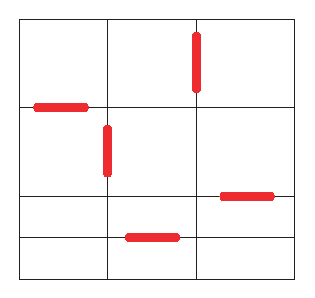
\includegraphics[scale=0.6]{figs/f4.illu-workflow-2d1.eps}
    \end{minipage}}
  \subfigure[]{
    \centering
    \label{fig:workflow2dortho:b}
    \begin{minipage}[b]{0.23\textwidth}
      \centering
      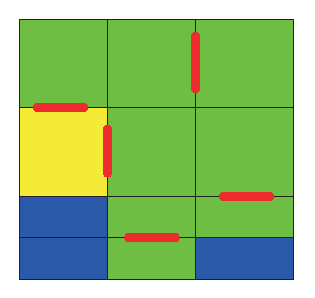
\includegraphics[scale=0.6]{figs/f4.illu-workflow-2d2.eps}
    \end{minipage}}
  \subfigure[]{
    \label{fig:workflow2dortho:c}
    \begin{minipage}[b]{0.23\textwidth}
      \centering
      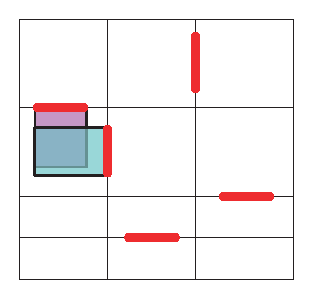
\includegraphics[scale=0.6]{figs/f4.illu-workflow-2d3.eps}
    \end{minipage}}
  \subfigure[]{
    \label{fig:workflow2dortho:d}
    \begin{minipage}[b]{0.23\textwidth}
      \centering
      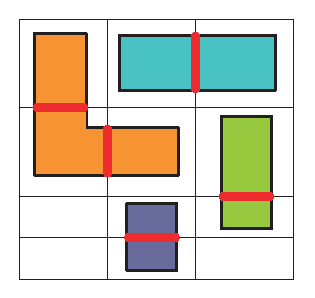
\includegraphics[scale=0.6]{figs/f4.illu-workflow-2d4.eps}
    \end{minipage}}
  \subfigure[]{
    \label{fig:workflow2dortho:e}
    \begin{minipage}[b]{0.23\textwidth}
      \centering
      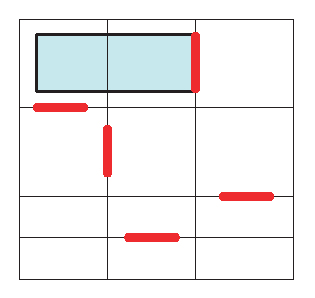
\includegraphics[scale=0.6]{figs/f4.illu-workflow-2d5.eps}
    \end{minipage}}
  \subfigure[]{
    \label{fig:workflow2dortho:f}
    \begin{minipage}[b]{0.23\textwidth}
      \centering
      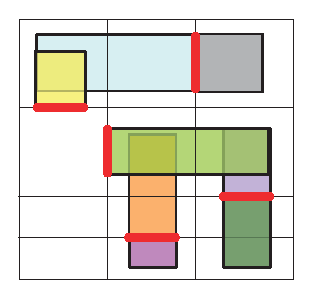
\includegraphics[scale=0.6]{figs/f4.illu-workflow-2d6.eps}
    \end{minipage}}
  \subfigure[]{
    \label{fig:workflow2dortho:g}
    \begin{minipage}[b]{0.23\textwidth}
      \centering
      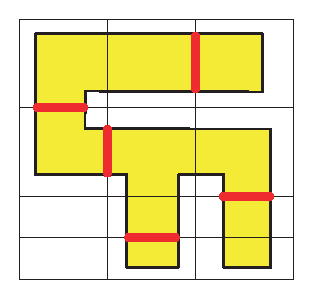
\includegraphics[scale=0.6]{figs/f4.illu-workflow-2d7.eps}
    \end{minipage}}
  \caption{2D illustration of our surface reconstruction algorithm.
  (a) Input segments (red, corresponding to the 3D cross sections) and partitioned zones;
  (b) The \textit{empty} zones (blue), \textit{end} zones (green) and \textit{body} zones (yellow);
  (c) Generating polygons (corresponding to the cylinders) in \textit{body} zones;
  (d) Generating polygons in the \textit{end} zones using the same way as the reconstruction in the \textit{body} zones. The reconstruction result contains multiple components;
  (e) Generating extended polygons for an \textit{end} zone;
  (f) Generating polygons for all \textit{end} zones;
  (g) The reconstruction result. }
  \label{fig:workflow2dortho}
\end{figure*}


%basic workflow
Similar to~\cite{LBDLJ08}, our algorithm also  follows the general
divide-and-conquer strategy. That is, we first place a large virtual
bounding box containing all the cross sections (we set its size to be 2 times
that of the bounding box of all points on the cross sections). This box will keep
fixed during the sketching process and all points on the input cross
sections will lie within it. Then we partition the box into zones
$ZN=\{zn_i~|~i=1,...,m\}$ using the planes that the cross sections
lie on. The shape of each zone $zn_i$ is thus a cuboid since we only
allows the translation of the orthogonal reference planes. Within
$zn_i$, the curves might be split into segments such that the segments
are entirely lie in the faces $F=\{f_{ij}~|~f_{ij}\in
zn_i,j=1,...,n\}$. Next we build a sub-surface which interpolates
the curve segments on the faces of each zone and stitch all the
pieces of sub-surfaces together to form a complete surface. Finally
we carry out constrained refinement and smoothing to the initial
mesh surface to improve its quality while maintaining its
interpolation on the input cross sections.

%limitation of TJ's method
Though the projection-based method in~\cite{LBDLJ08} can be used for
reconstruction, it will make the shape of the reconstructed surface
rely on that of the geometric agency (the MA plane) to a large
extent. In the progressive modeling process, each time a new cross
section is sketched on a new plane, the MA planes in the related
zones will be re-calculated, which probably leads to the shape
change of the surface components generated from all the cross
sections within these zones, and further the change of the
sub-surfaces. In that case, some surface parts generated from some
unrelated cross sections will be changed, resulting in unexpected
shape changes of the model surface. Especially in the iterative
sketching process, different input orders of a same set of sketched
curves will introduce different changes of the agencies, and the
shape changes will be unexpected under some input orders of the
curves. In other words, whether gradual shape changes can be
achieved or not depends on the sketching orders to some extent. Such
an example is shown in Figure~\ref{fig:csgma}. When new cross
sections are added following the order in Figure~\ref{fig:csgma:a},
unexpected shape change (breaking the originally connected
component) happened, which obviously goes against user's intention.

\begin{figure*} [htbp]
  \centering
  \subfigure[]{
    \centering
    \label{fig:csgma:a} %% label for first subfigure
    \begin{minipage}[b]{0.18\textwidth}
      \centering
      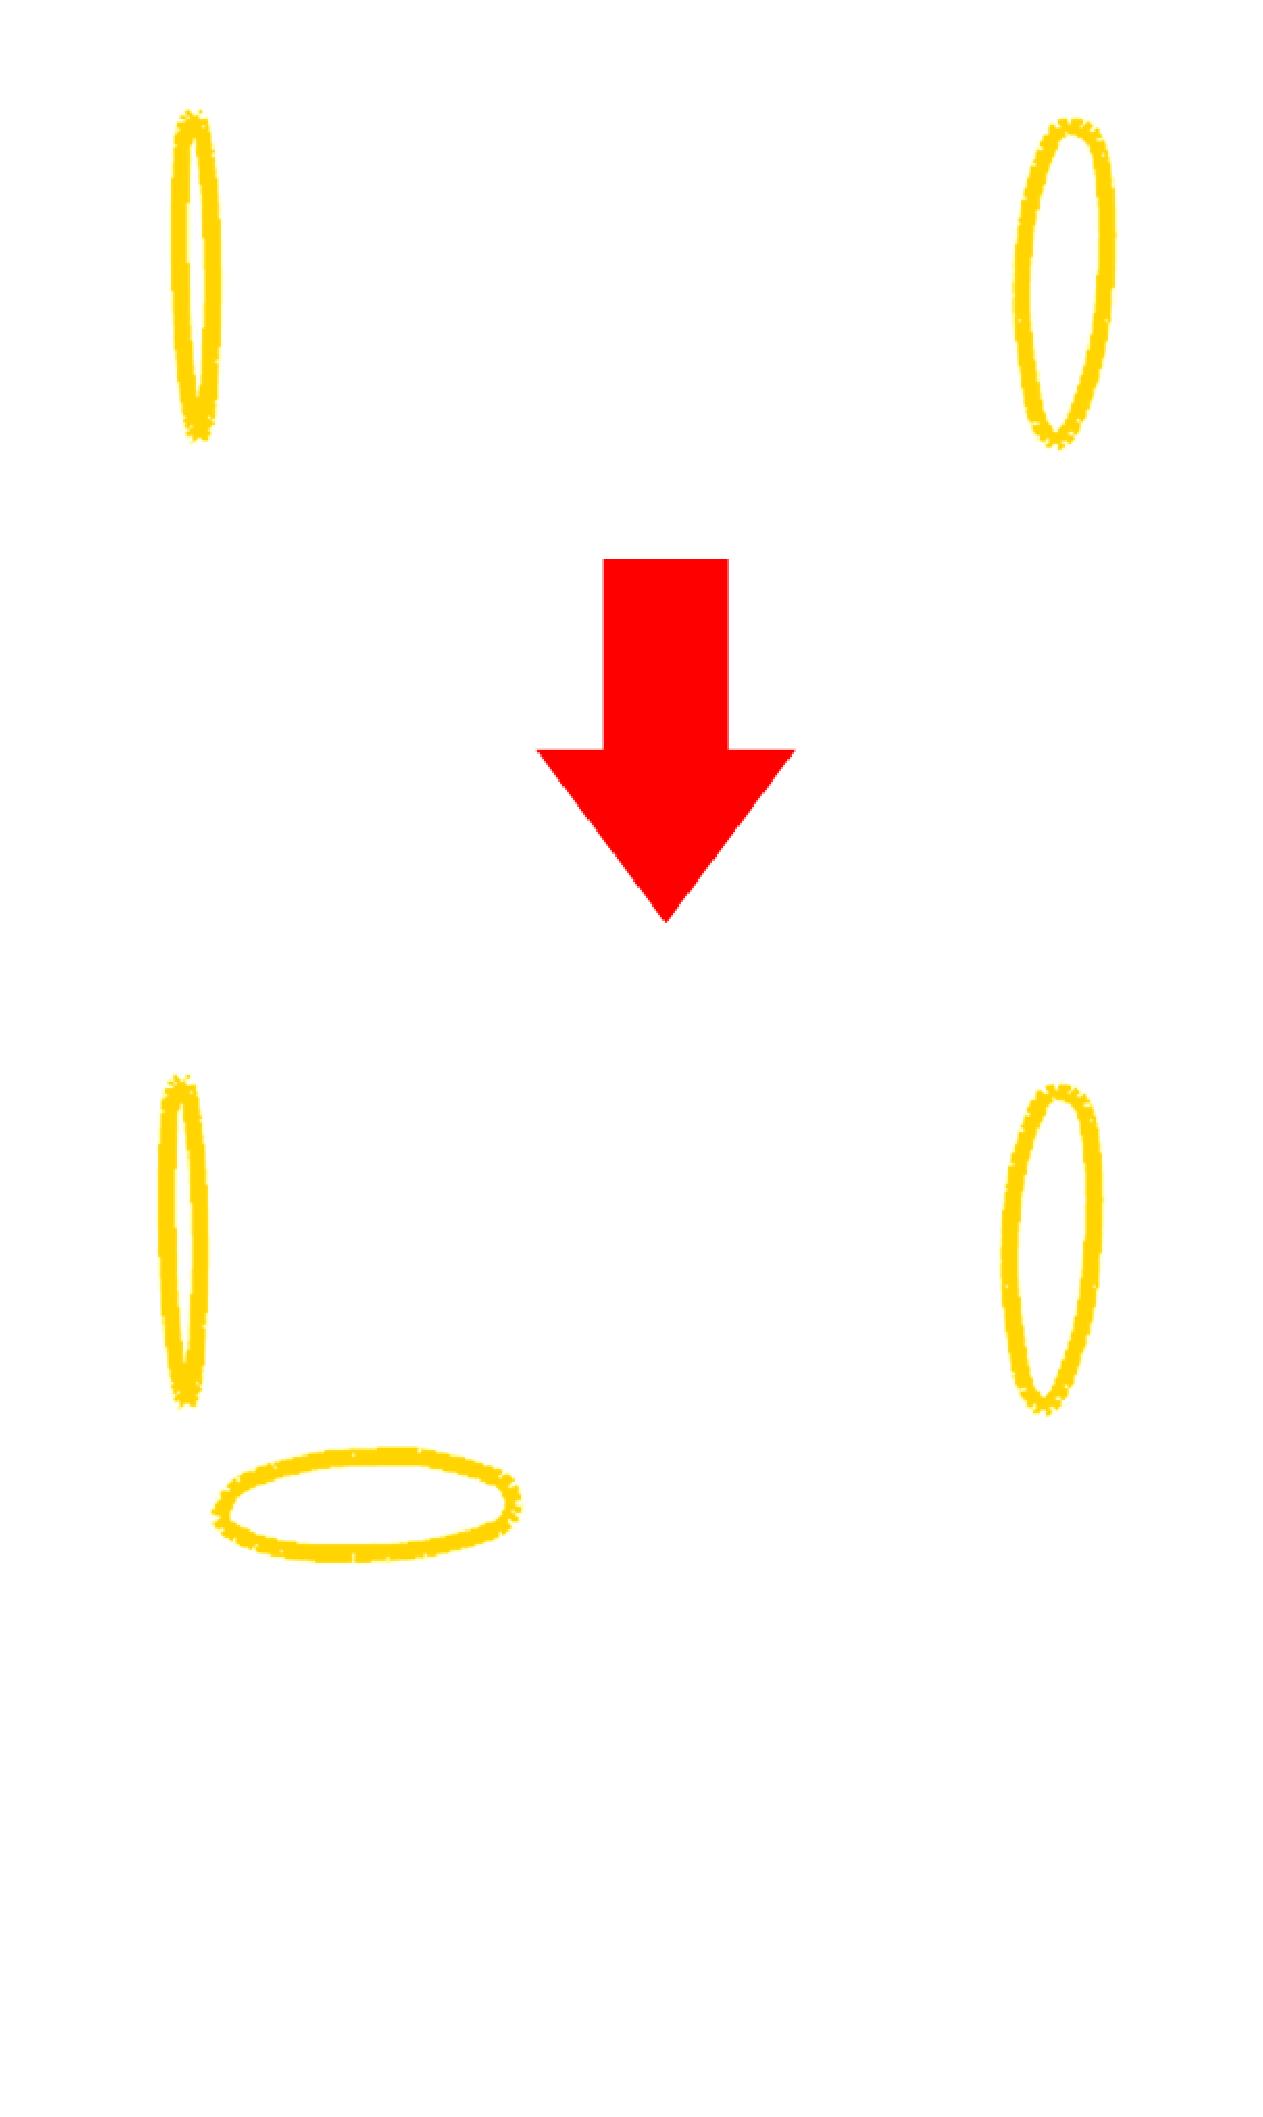
\includegraphics[scale=0.12]{figs/f3.surf-csgma-1.eps}
    \end{minipage}}
  \subfigure[]{
    \centering
    \label{fig:csgma:b}
    \begin{minipage}[b]{0.18\textwidth}
      \centering
      \includegraphics[scale=0.12]{figs/f3.surf-csgma-2.eps}
    \end{minipage}}
  \subfigure[]{
    \centering
    \label{fig:csgma:c}
    \begin{minipage}[b]{0.18\textwidth}
      \centering
      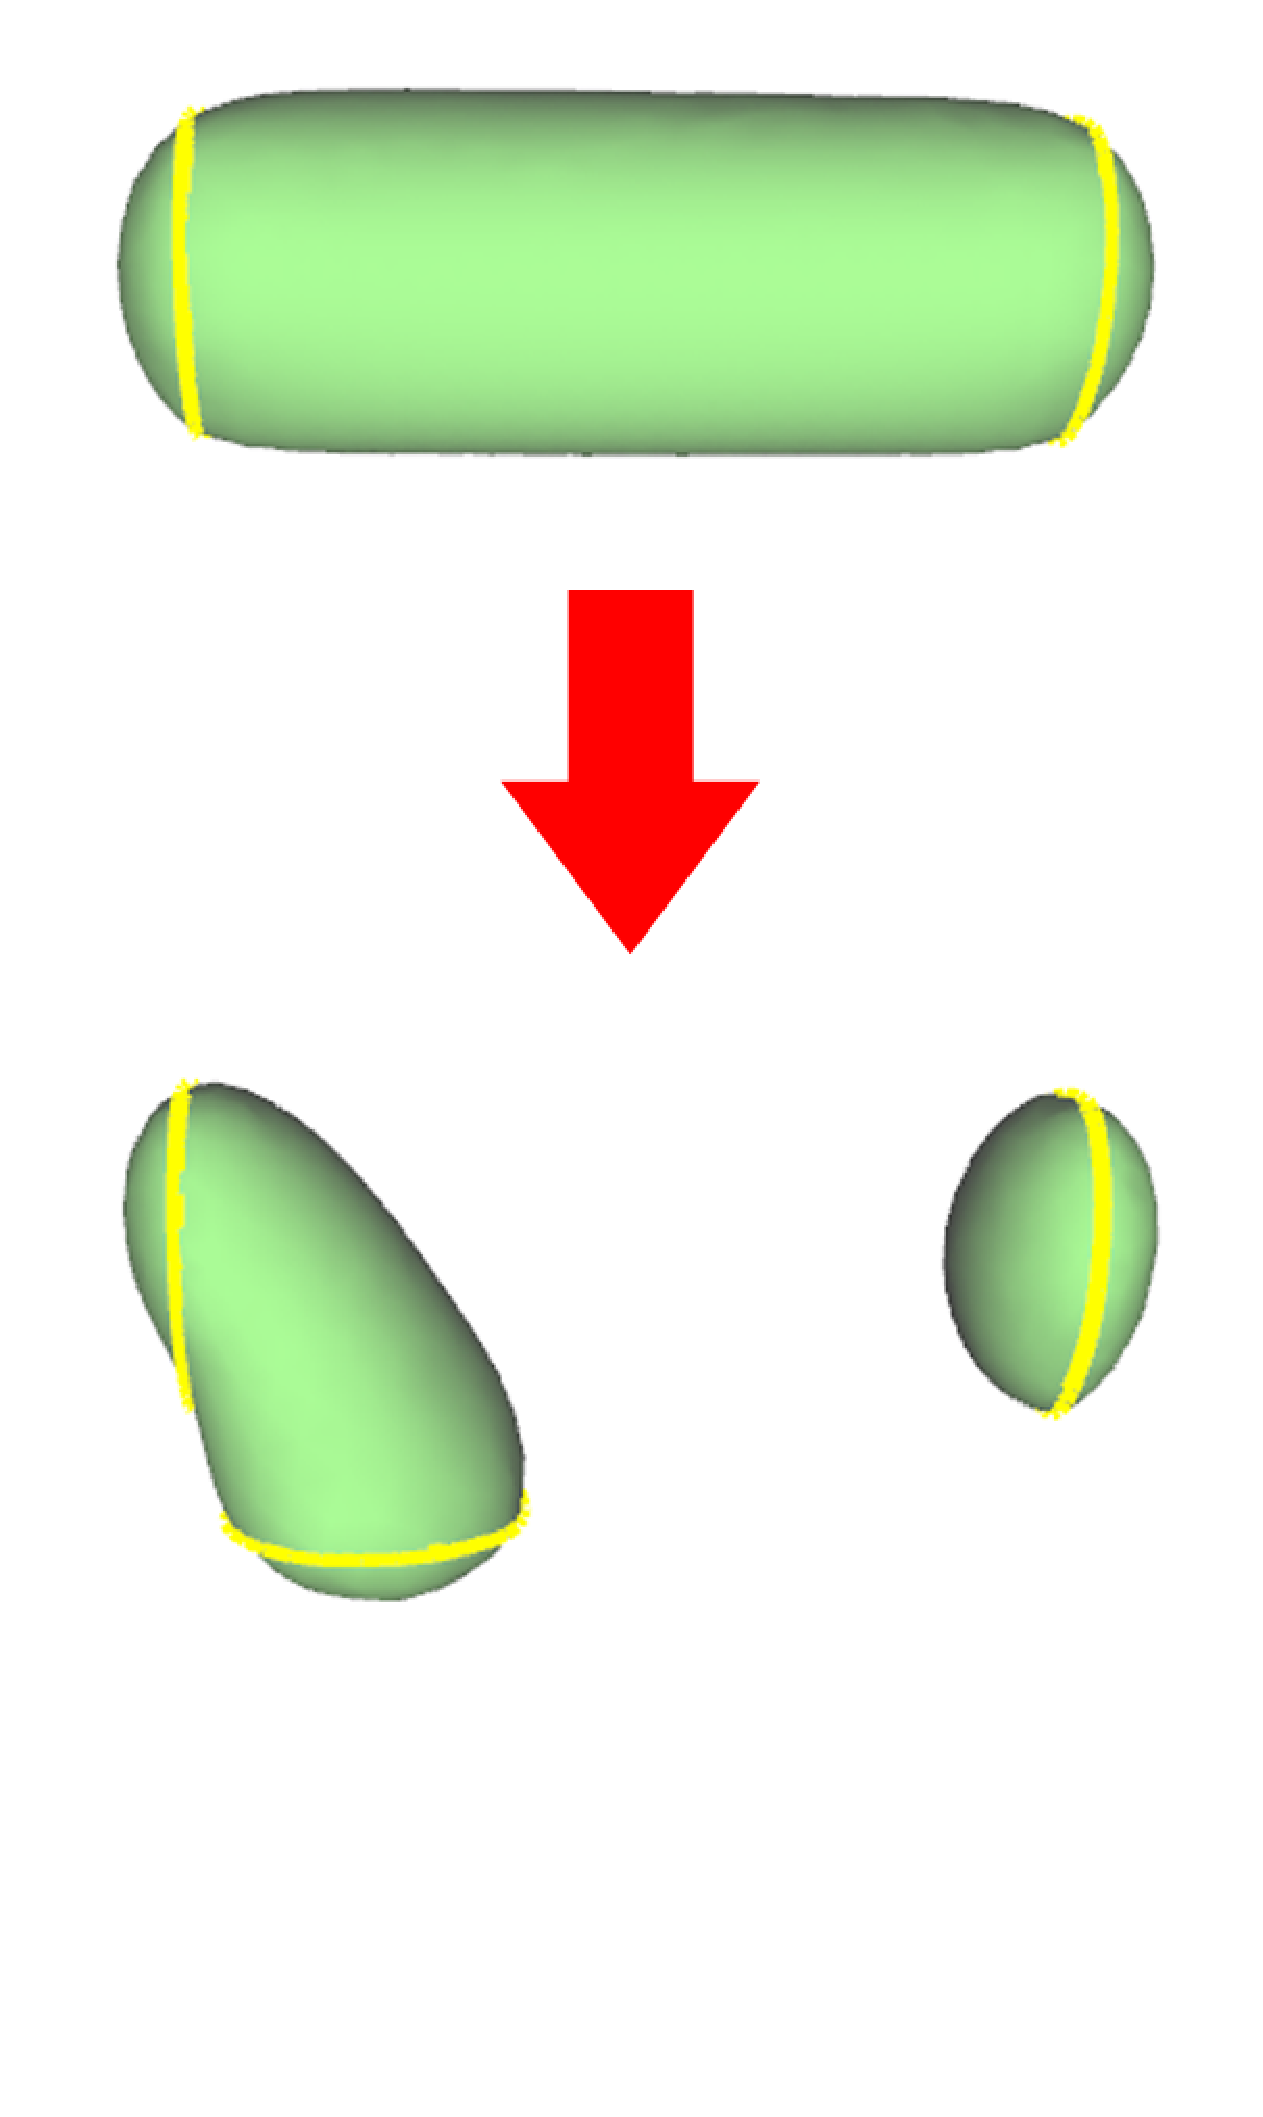
\includegraphics[scale=0.12]{figs/f3.surf-csgma-3.eps}
    \end{minipage}}
  \subfigure[]{
    \centering
    \label{fig:csgma:d}
    \begin{minipage}[b]{0.18\textwidth}
      \centering
      \includegraphics[scale=0.12]{figs/f3.surf-csgma-4.eps}
    \end{minipage}}
  \subfigure[]{
    \centering
    \label{fig:csgma:e}
    \begin{minipage}[b]{0.18\textwidth}
      \centering
      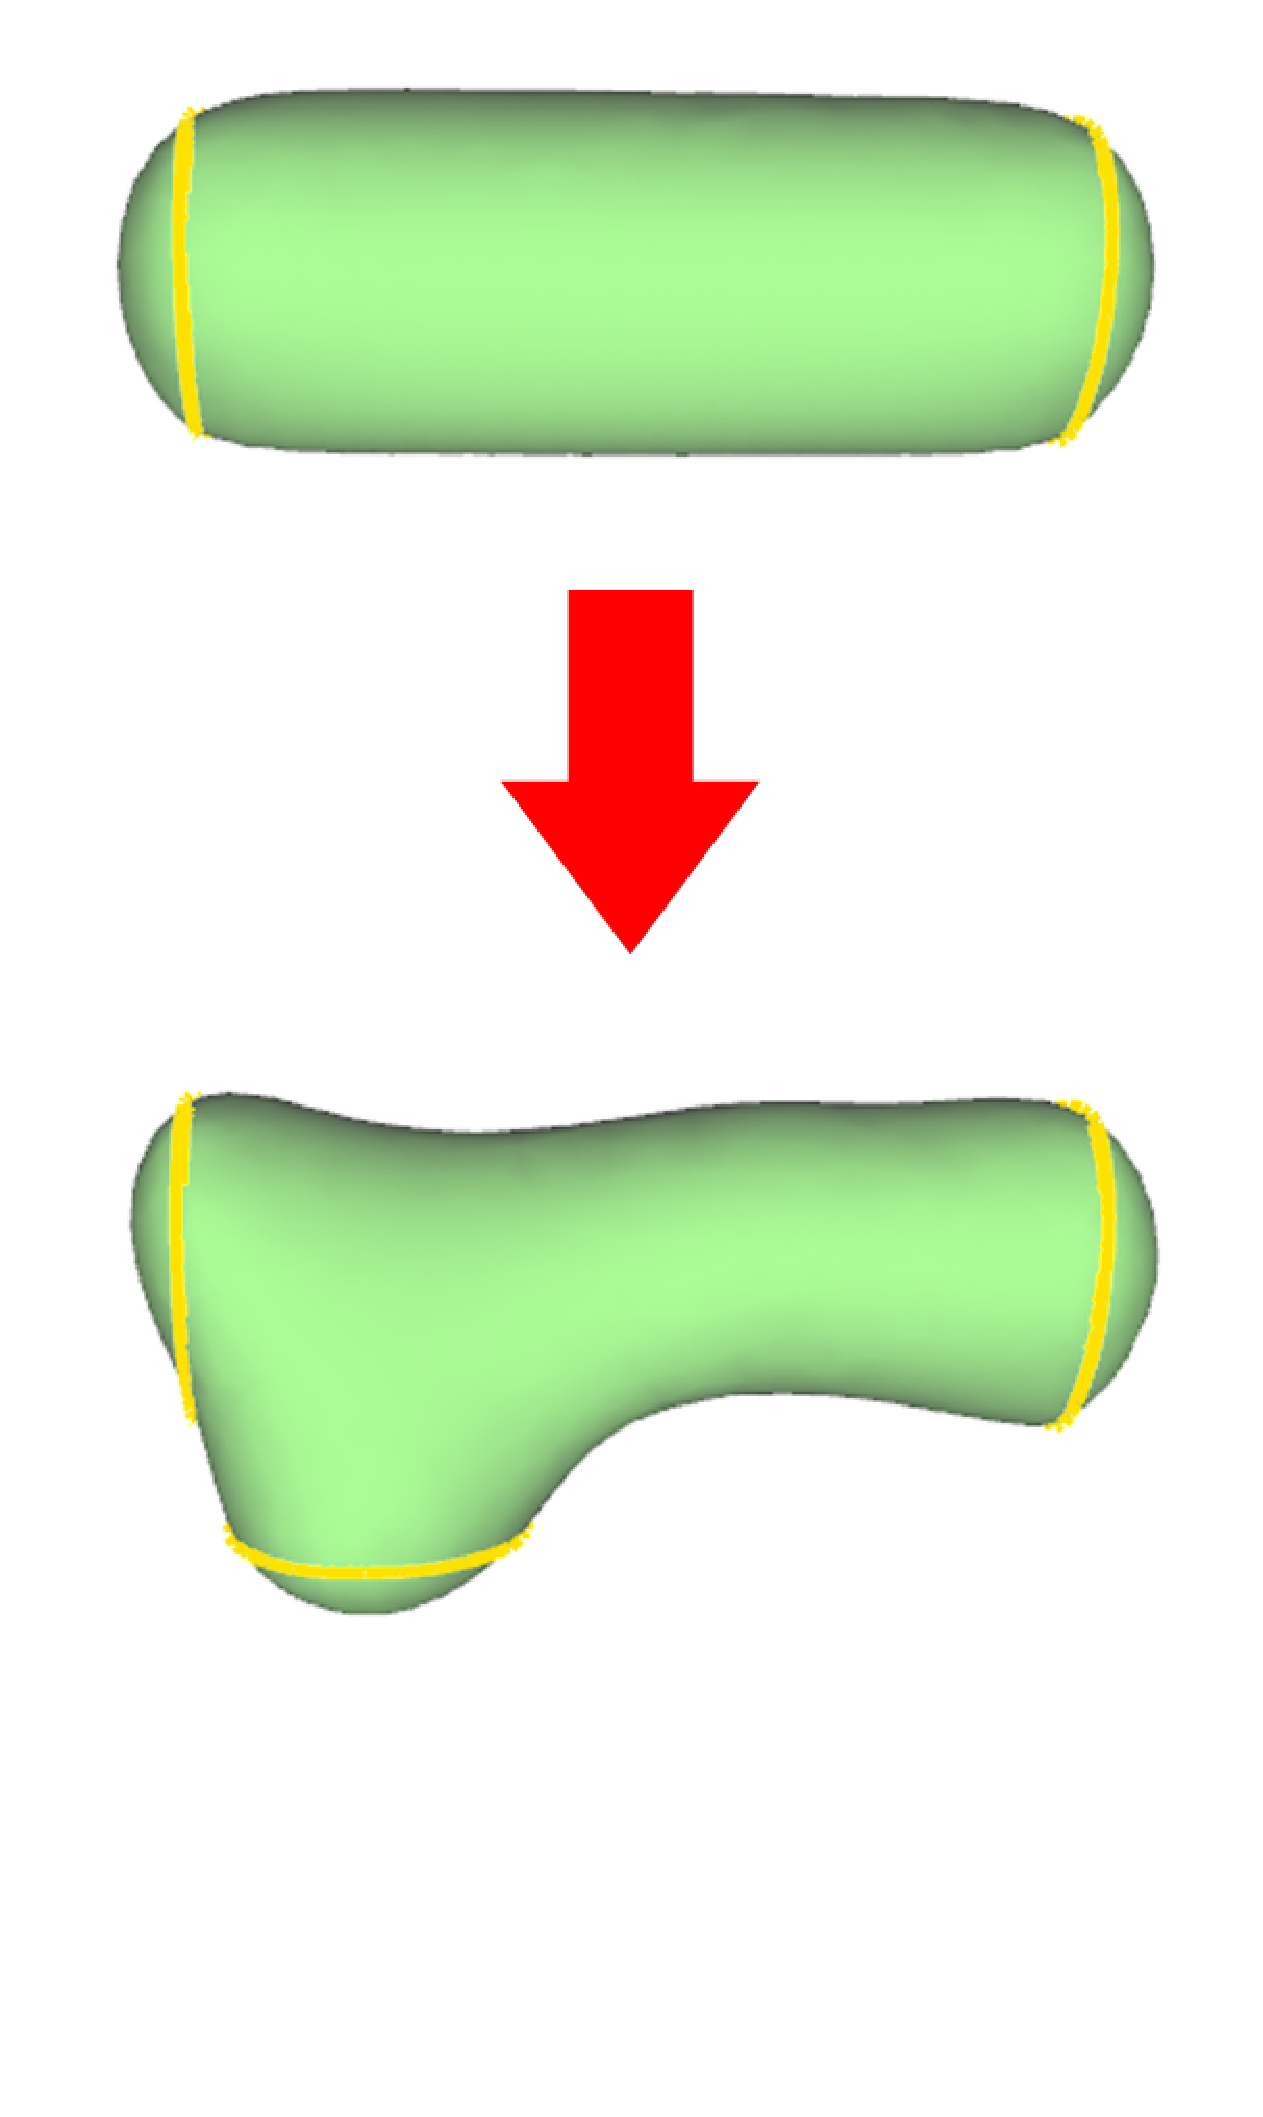
\includegraphics[scale=0.12]{figs/f3.surf-csgma-5.eps}
    \end{minipage}}
  \caption{An example of comparing our surface reconstruction algorithm  and that of~\cite{LBDLJ08}. (a) Two cross sections are sketched first and then one more is added; (b) The initial reconstruction results in~\cite{LBDLJ08}. The Medial Axis planes (blue) in a zone are shown; (c) The final reconstruction results in~\cite{LBDLJ08}; (d) The initial reconstruction results in our algorithm. The union of cylinders in each zone is shown; (e) The final reconstruction results in our algorithm.}
  \label{fig:csgma} %% label for entire figure
\end{figure*}

%motivation of the csg method
To get rid of the affection of the geometric agency and produce
gradual shape change during progressive modeling, we used a CSG
(Constructive Solid Geometry)-based method, instead of the
projection-based method to generate the sub-surface in each zone.
Our method is inspired by the work~\cite{RDI10}, which builds a 3D
model from 2D silhouettes sketched under orthogonal views by
generating cylinders from each silhouette and computing the union of
them. However, the inputs in our system are 3D cross sections with
different depths and complex mutual relationship, so the computation
will be more involved.

%csg method
Generally, in each zone $zn_i$, we build a cylinder from  each cross
section $cs_p$ and then compute the union of these cylinders.
Meanwhile, we extend some cylinders which may probably become
isolated surface components, to make them intersect with cylinders
in other zones and thus reduce the possibility of the existence of
multiple components of the final surface. The final surface is then
obtained by stitching all pieces of the sub-surfaces built in each
zone.

%zone types
Specifically, depending on the number of faces  having cross section
curves on, a zone is first classified into one of the following
three types:
\begin{itemize}
    \item A zone with no faces containing cross sections (denoted by an \textit{empty} zone),
    \item A zone with only one face containing cross sections (denoted by an \textit{end} zone),
    \item A zone with two or more faces containing cross sections (denoted by a \textit{body} zone).
\end{itemize}
Figure~\ref{fig:workflow2dortho} is a 2D illustration of such a
partition with three types of zones. The red segments on the lines
correspond to the cross sections on the zone faces.


In the next three sections, we will show how to create sub-surfaces in
the \textit{body} zones and \textit{end} zones and how to stitch
the sub-surfaces. For an \textit{empty} zone, it has no cross
sections and is thus ignored.




\section{Sub-surface reconstruction for a \textit{body} zone}
\label{ch4:sec:algo:body}

\begin{figure*} [htbp]
  \centering
  \subfigure[]{
    \centering
    \label{fig:cshape:a} %% label for first subfigure
    \begin{minipage}[b]{0.22\textwidth}
      \centering
      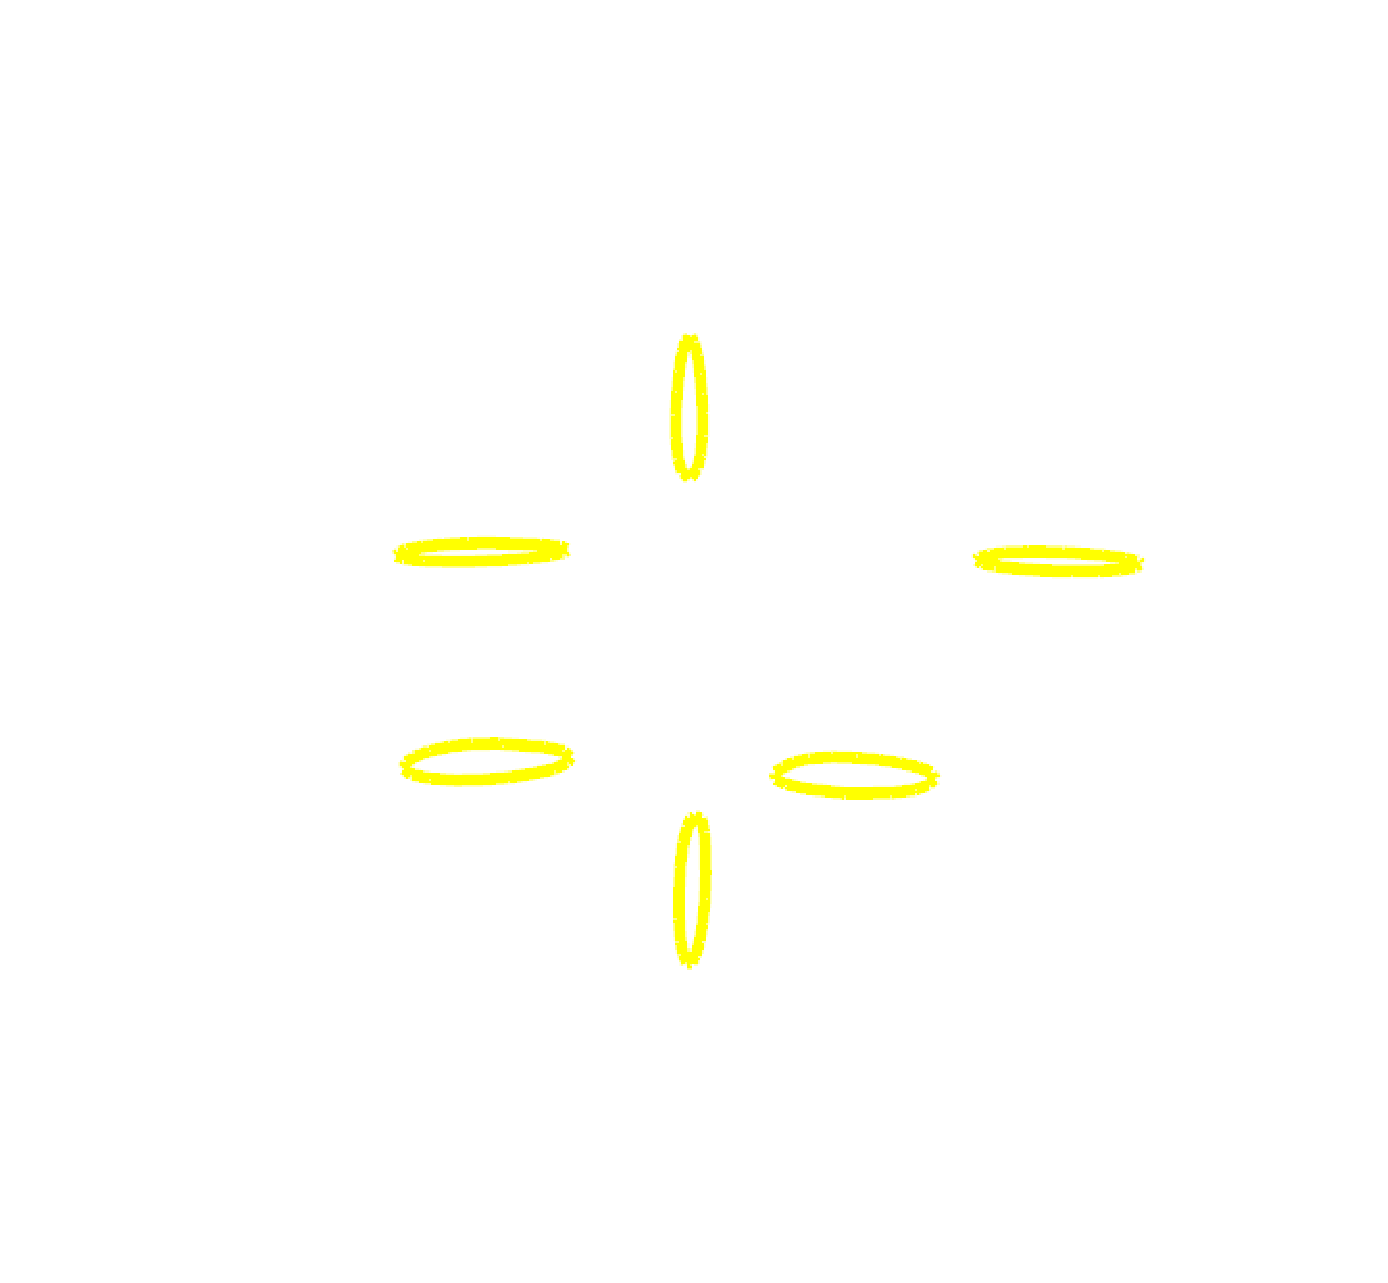
\includegraphics[scale=0.15]{figs/f3.surf-cshape-1.eps}
    \end{minipage}}
  \subfigure[]{
    \centering
    \label{fig:cshape:b}
    \begin{minipage}[b]{0.22\textwidth}
      \centering
      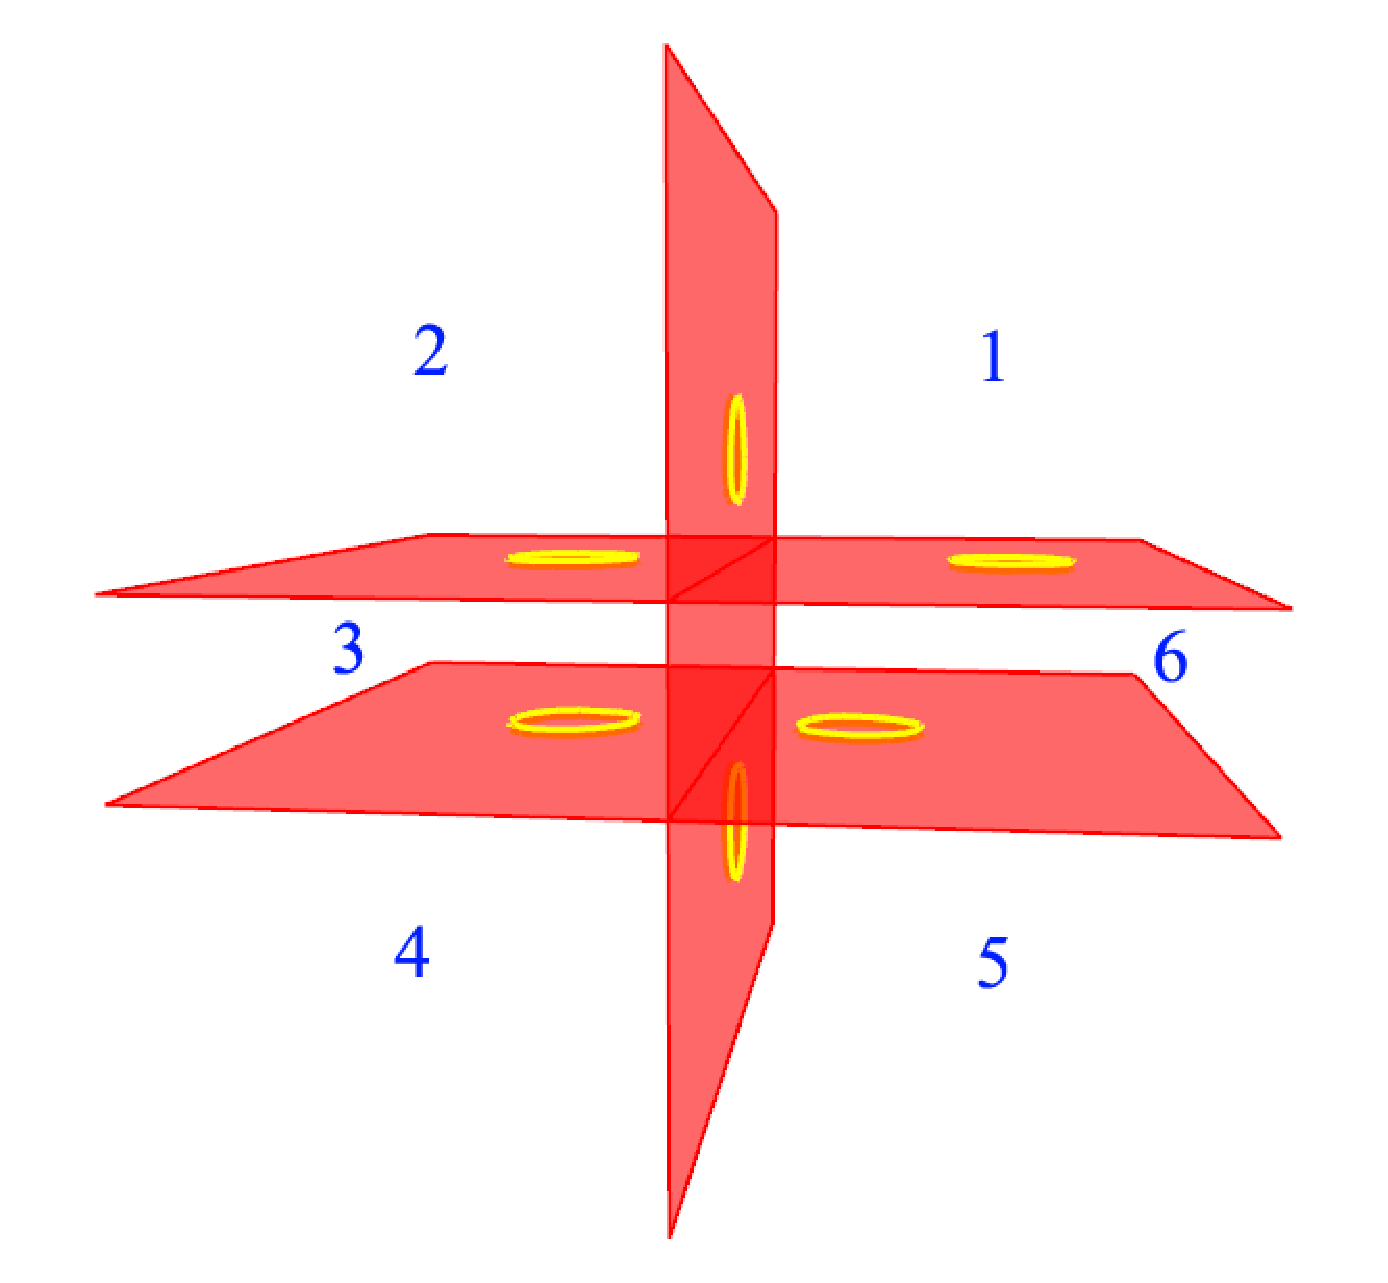
\includegraphics[scale=0.15]{figs/f3.surf-cshape-2.eps}
    \end{minipage}}
  \subfigure[]{
    \centering
    \label{fig:cshape:c}
    \begin{minipage}[b]{0.22\textwidth}
      \centering
      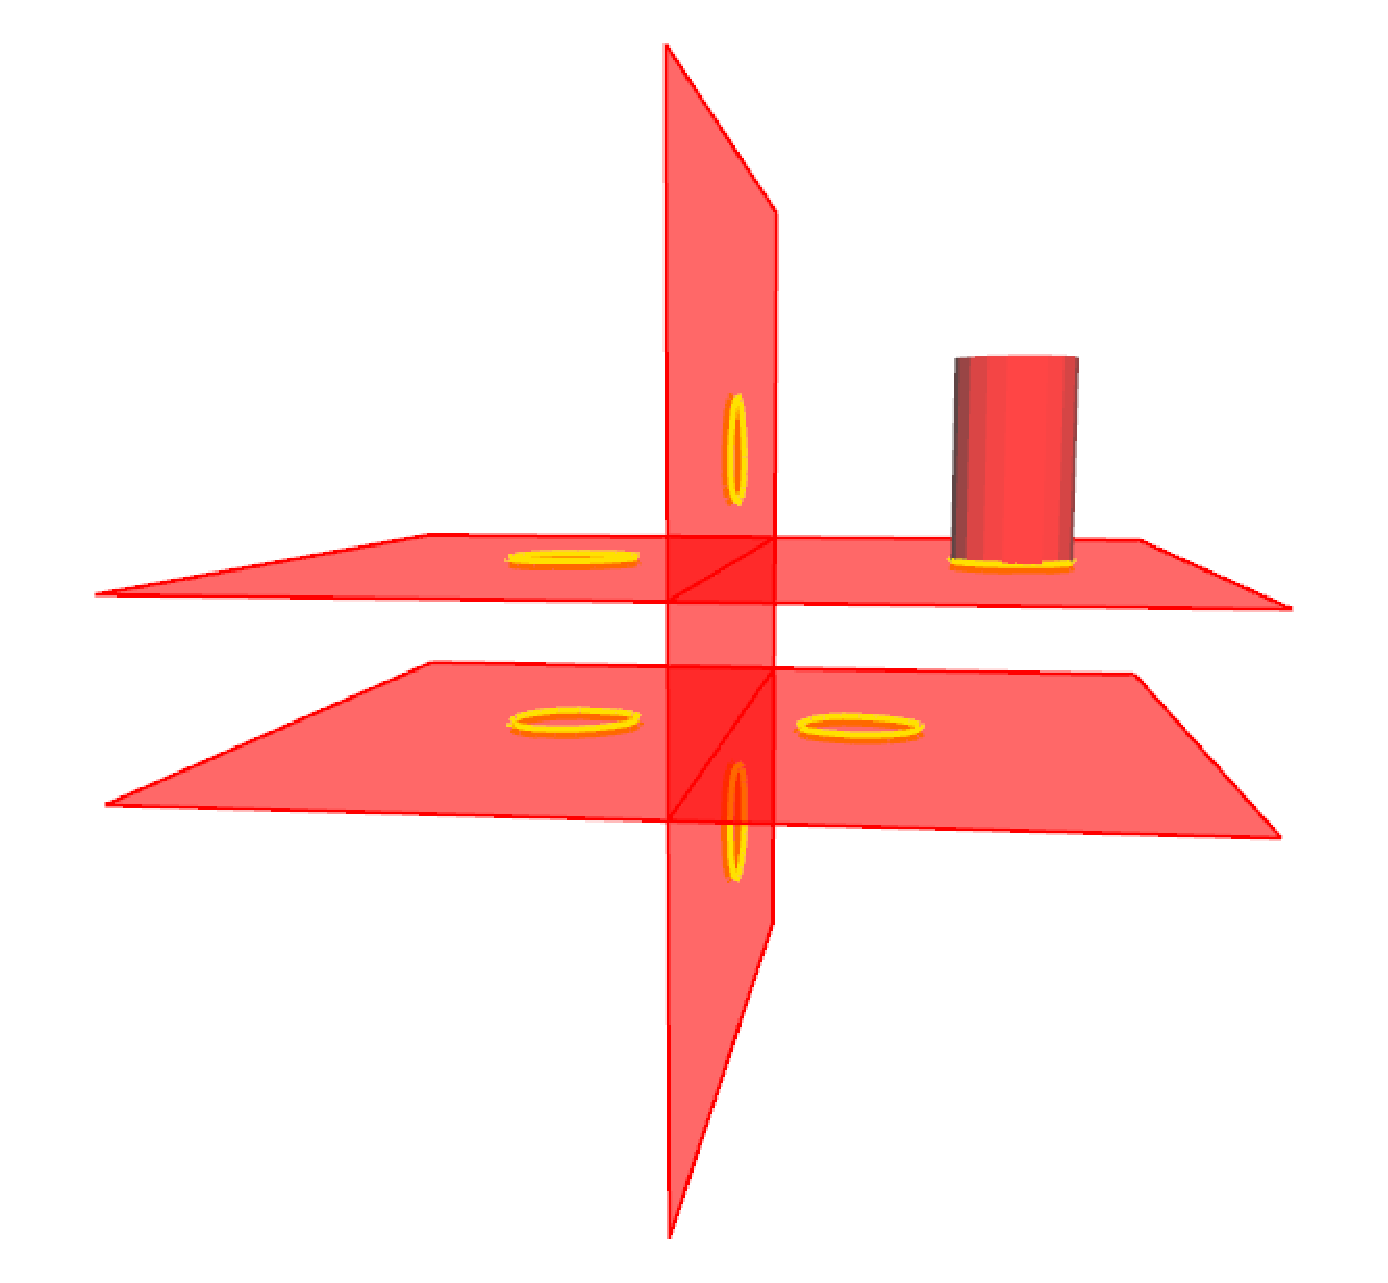
\includegraphics[scale=0.15]{figs/f3.surf-cshape-3.eps}
    \end{minipage}}
  \subfigure[]{
    \label{fig:cshape:d}
    \begin{minipage}[b]{0.22\textwidth}
      \centering
      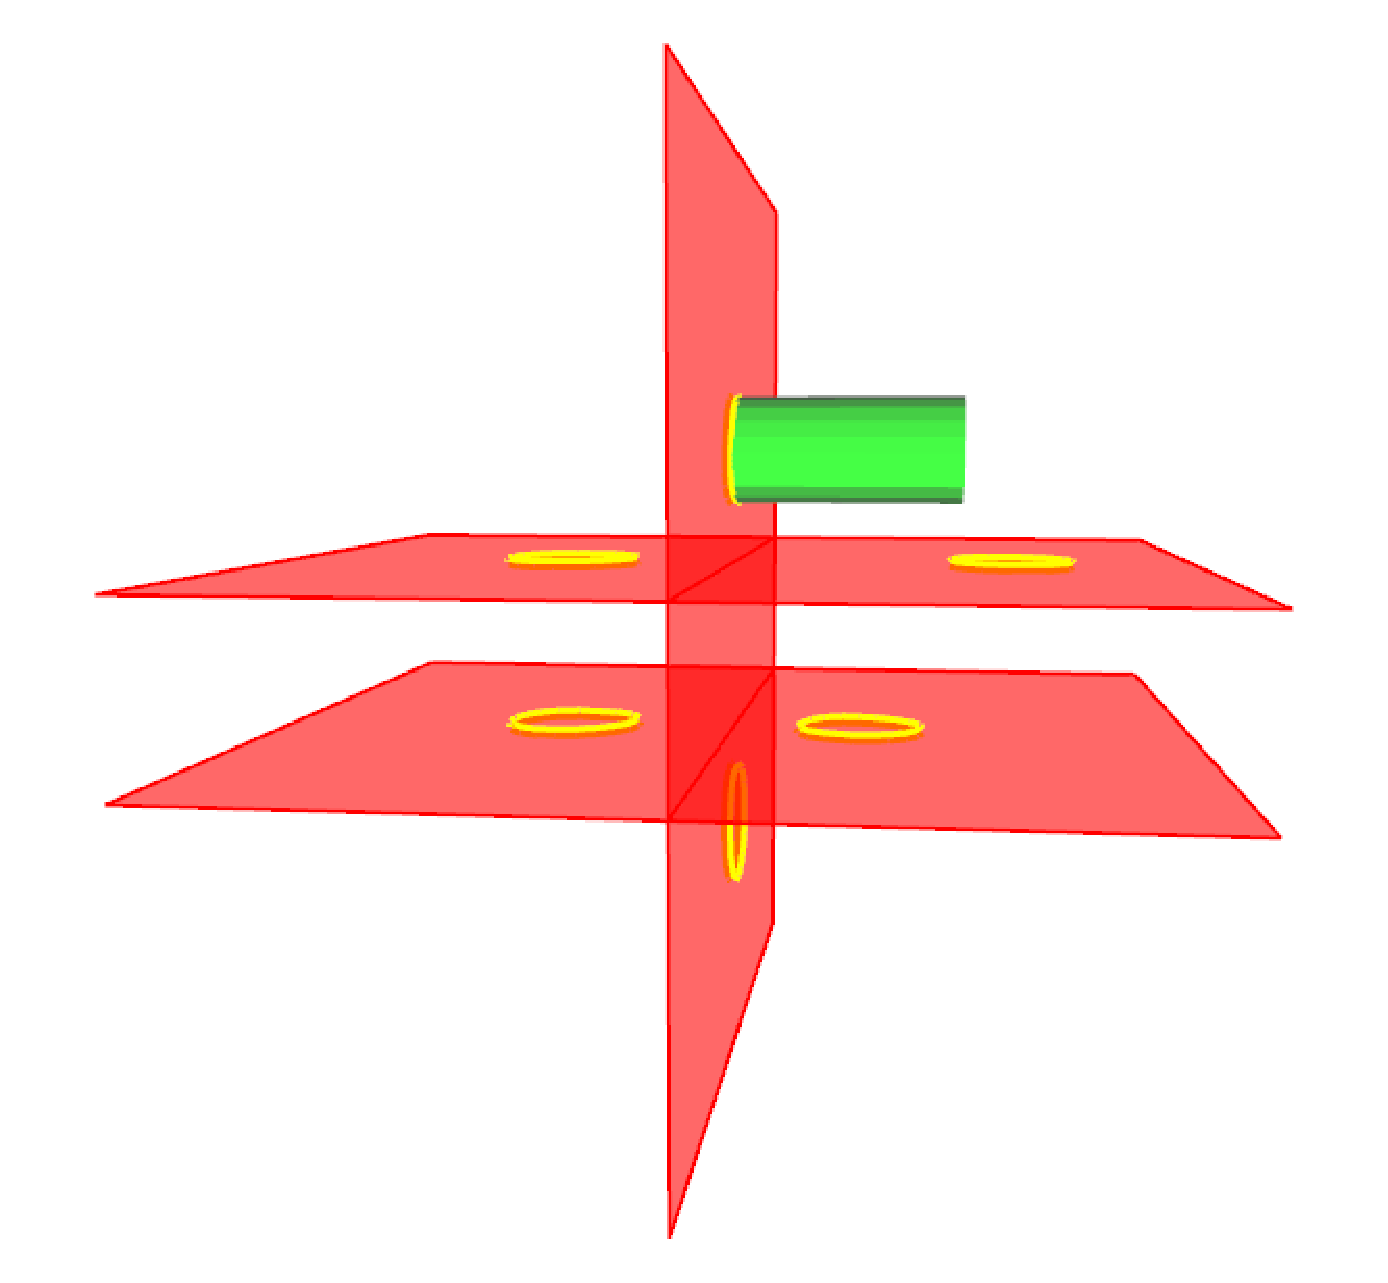
\includegraphics[scale=0.15]{figs/f3.surf-cshape-4.eps}
    \end{minipage}}
  \subfigure[]{
    \label{fig:cshape:e}
    \begin{minipage}[b]{0.22\textwidth}
      \centering
      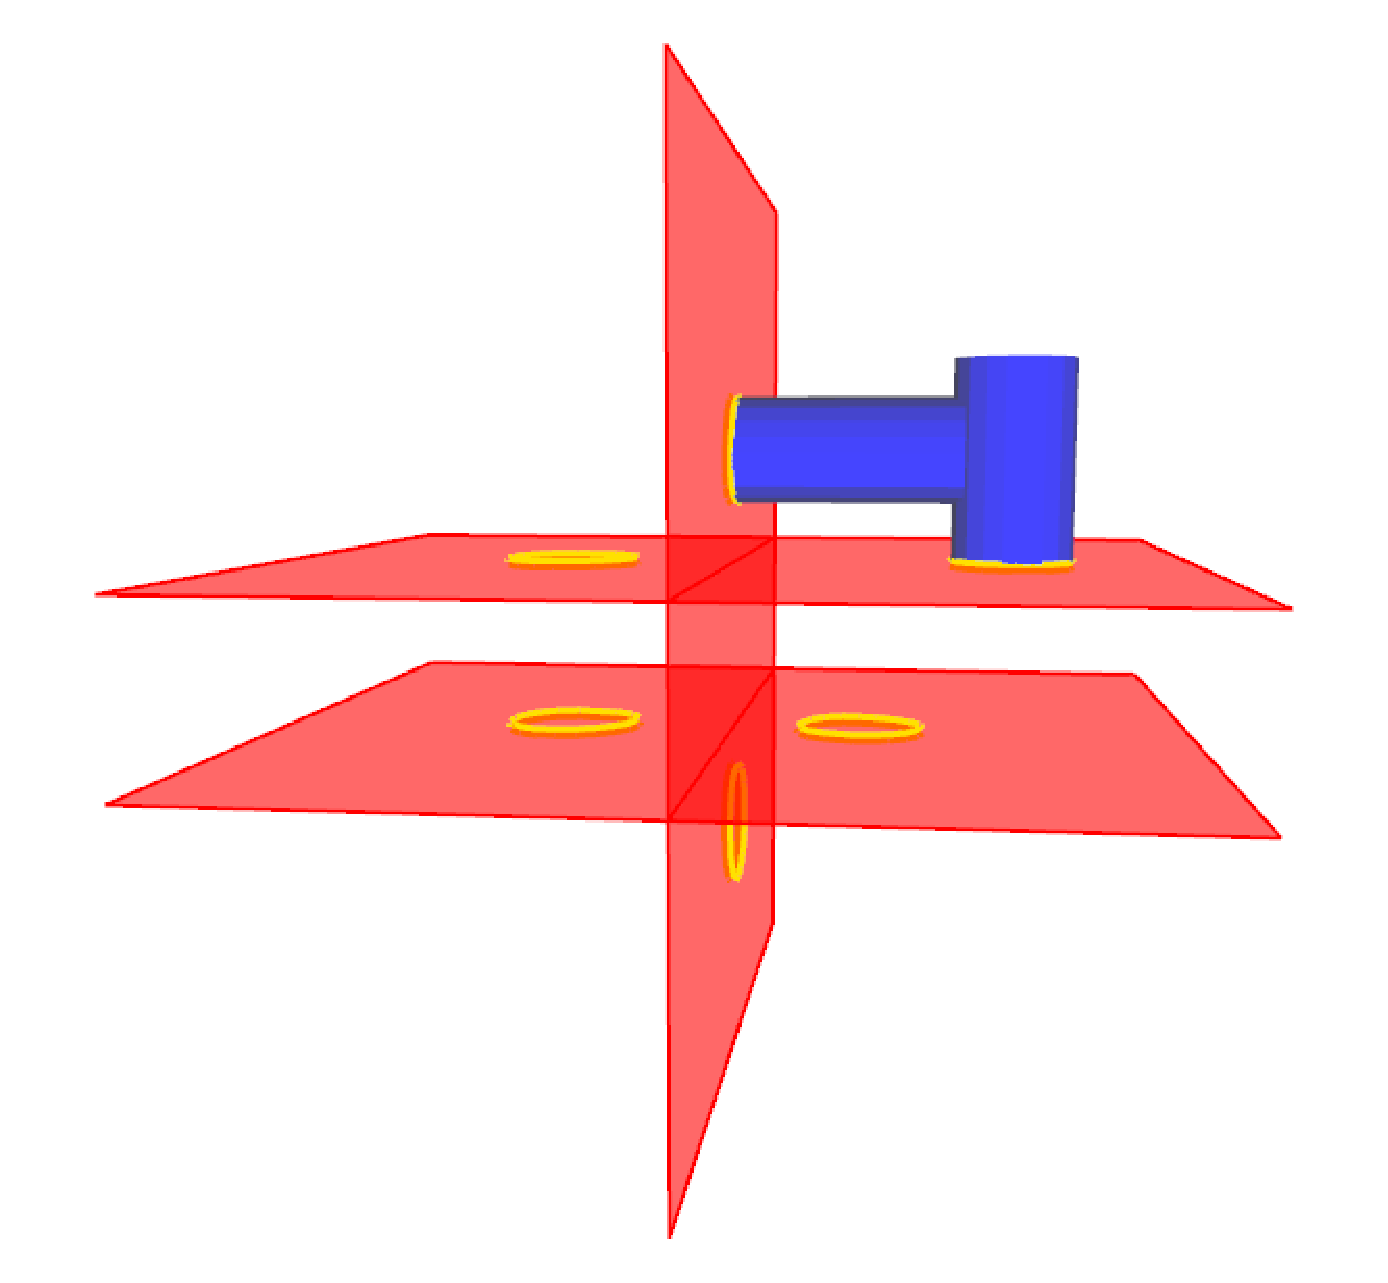
\includegraphics[scale=0.15]{figs/f3.surf-cshape-5.eps}
    \end{minipage}}
  \subfigure[]{
    \label{fig:cshape:f}
    \begin{minipage}[b]{0.22\textwidth}
      \centering
      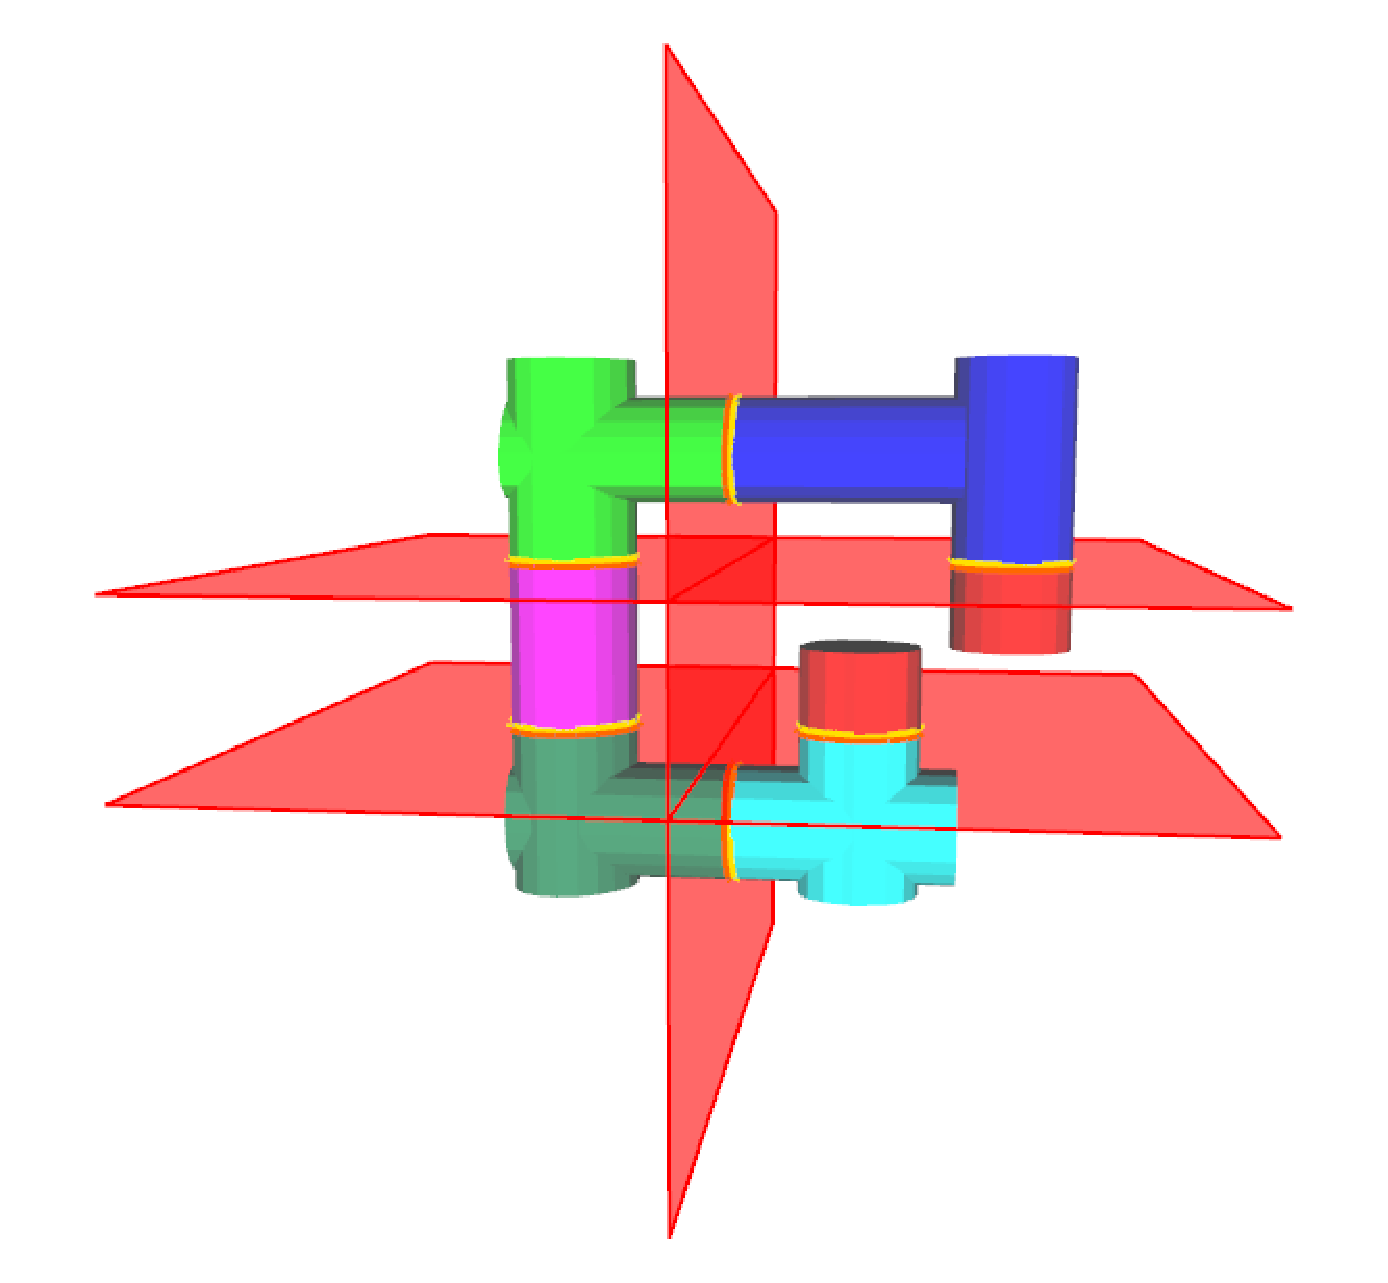
\includegraphics[scale=0.15]{figs/f3.surf-cshape-6.eps}
    \end{minipage}}
  \subfigure[]{
    \label{fig:cshape:g}
    \begin{minipage}[b]{0.22\textwidth}
      \centering
      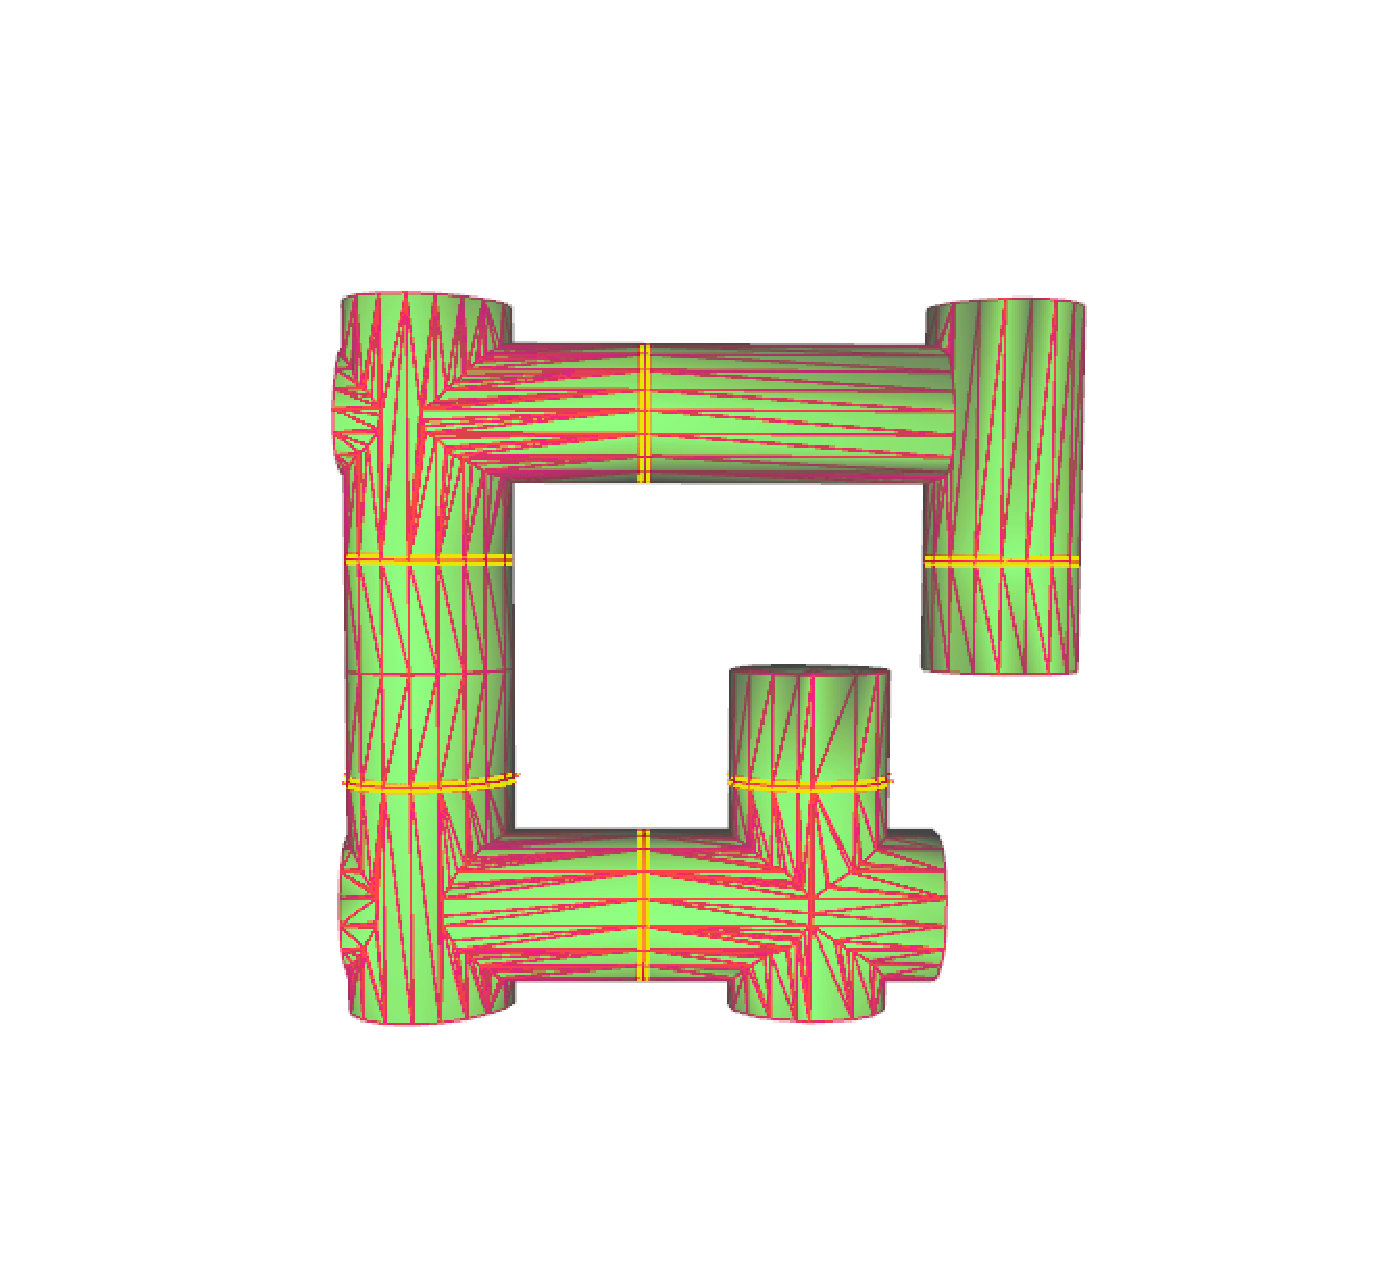
\includegraphics[scale=0.18]{figs/f3.surf-cshape-7.eps}
    \end{minipage}}
  \\
  \subfigure[]{
    \label{fig:cshape:h}
    \begin{minipage}[b]{0.22\textwidth}
      \centering
      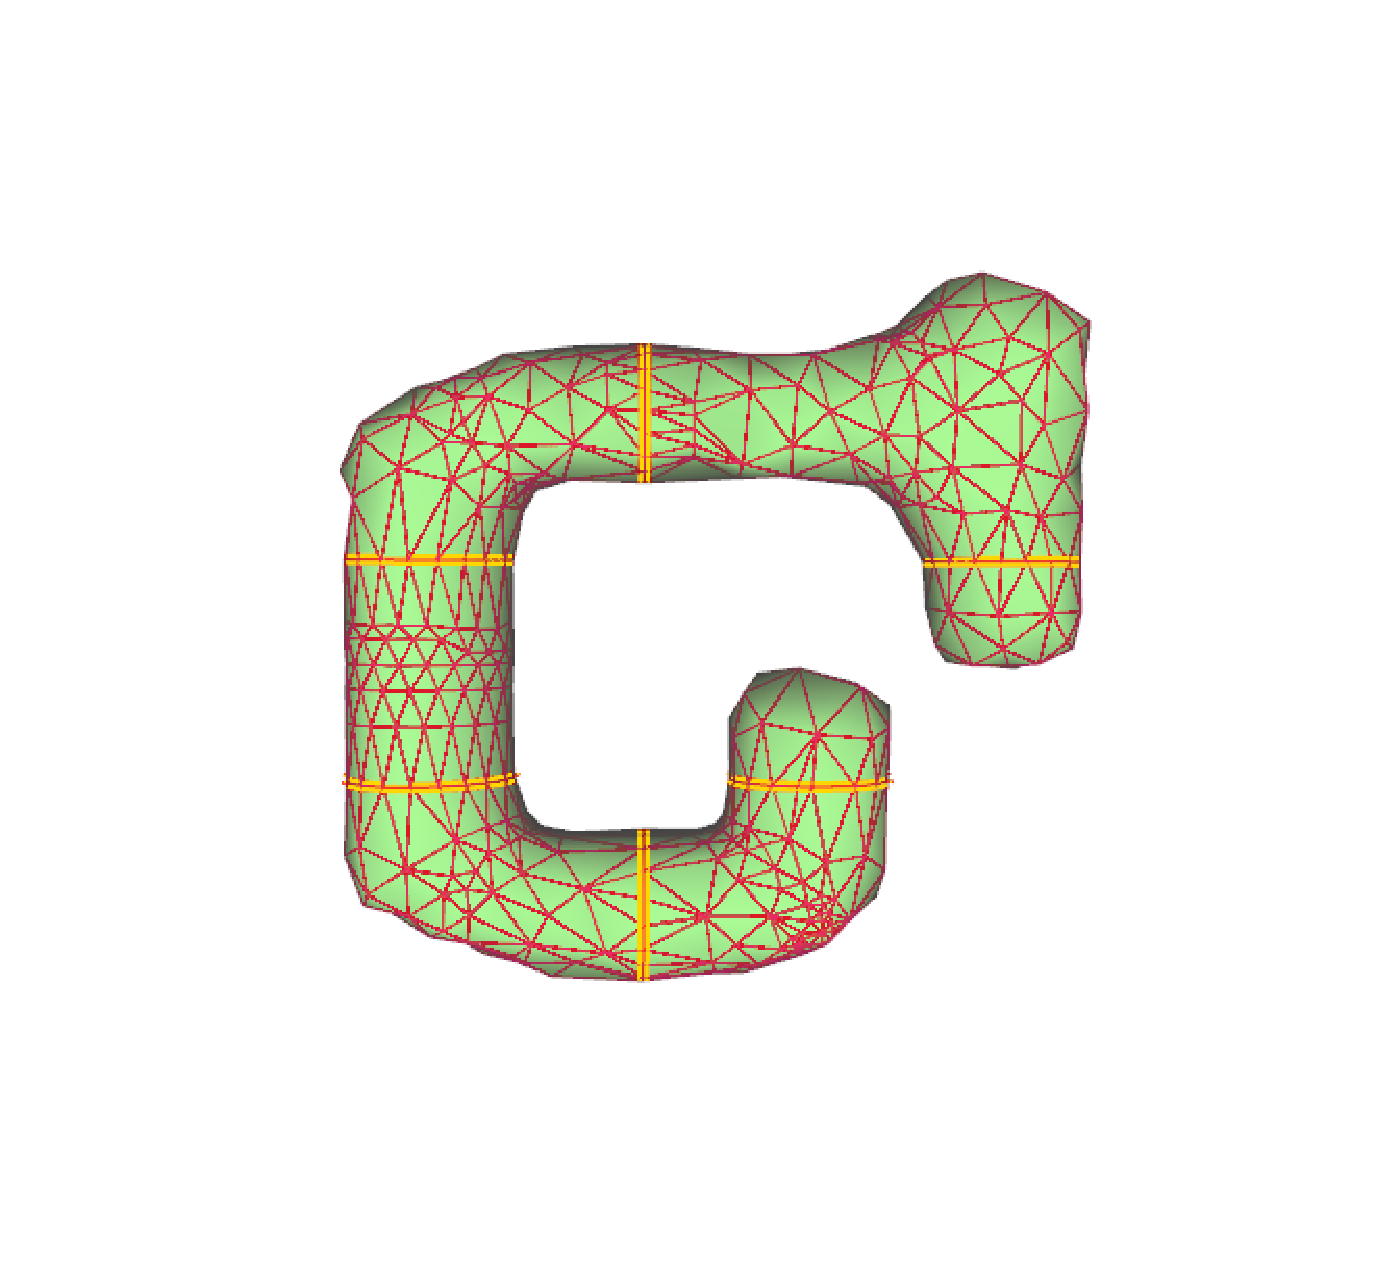
\includegraphics[scale=0.18]{figs/f3.surf-cshape-RS2.eps}
    \end{minipage}}
  \subfigure[]{
    \label{fig:cshape:i}
    \begin{minipage}[b]{0.22\textwidth}
      \centering
      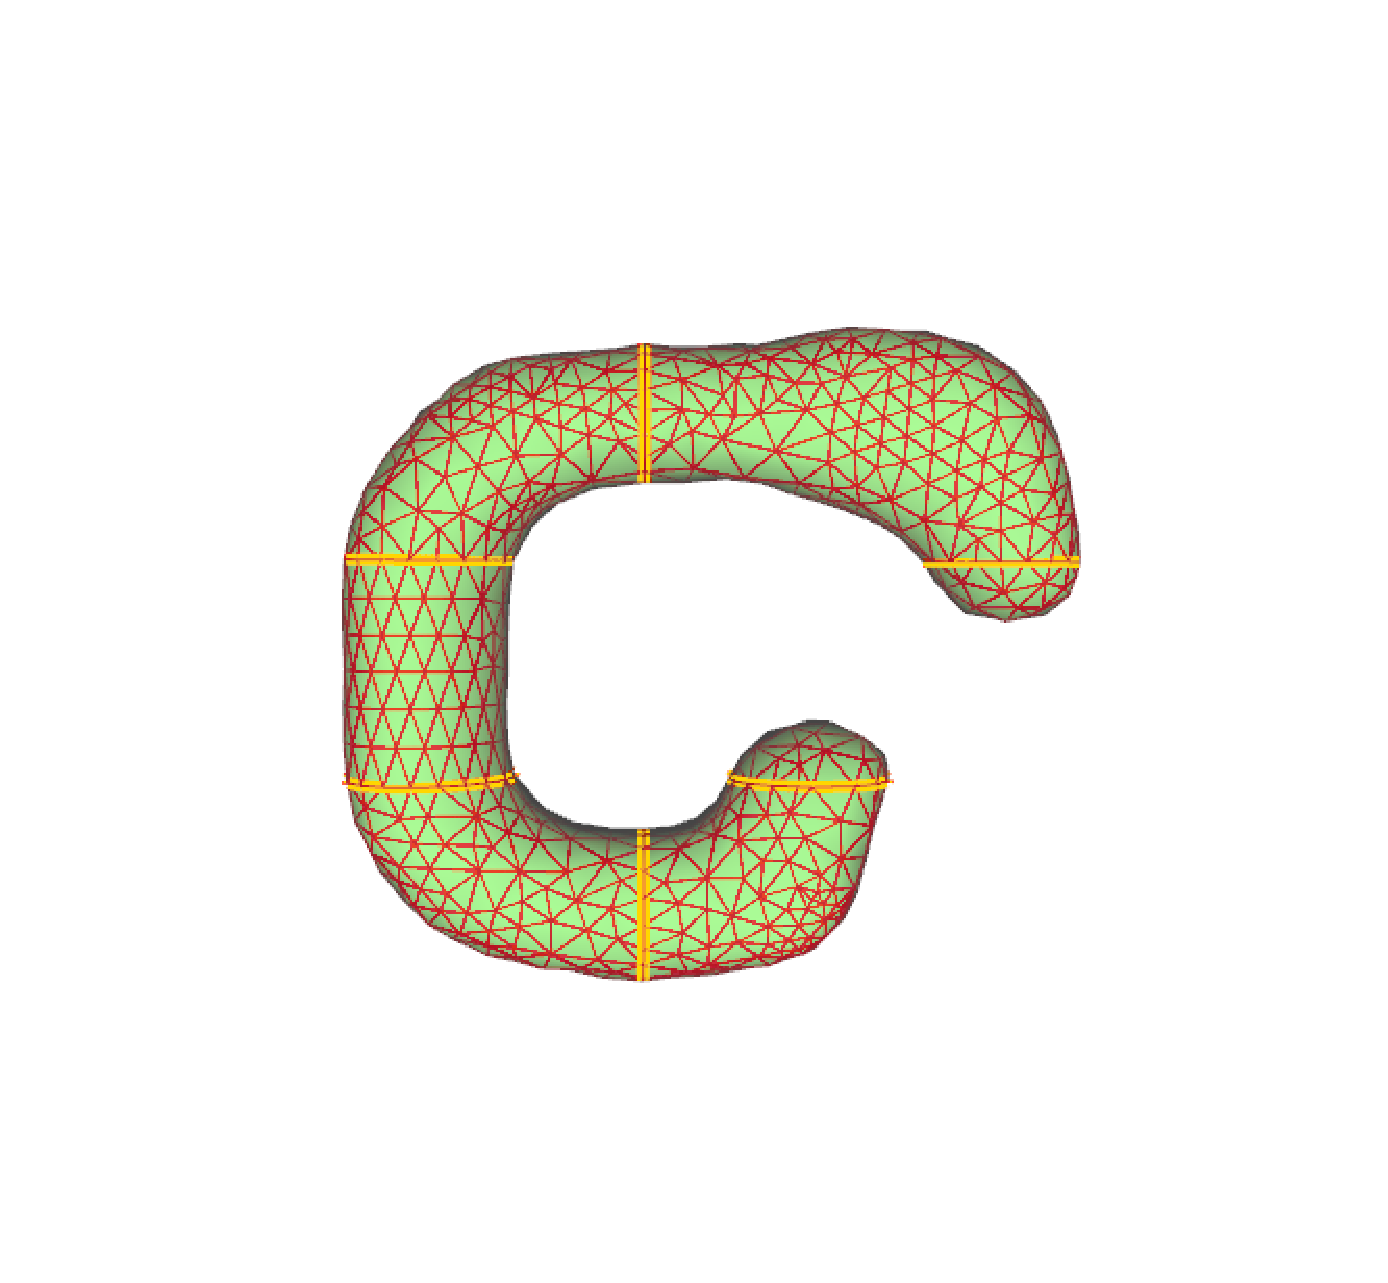
\includegraphics[scale=0.18]{figs/f3.surf-cshape-RS5.eps}
    \end{minipage}}
  \subfigure[]{
    \label{fig:cshape:j}
    \begin{minipage}[b]{0.52\textwidth}
      \centering
      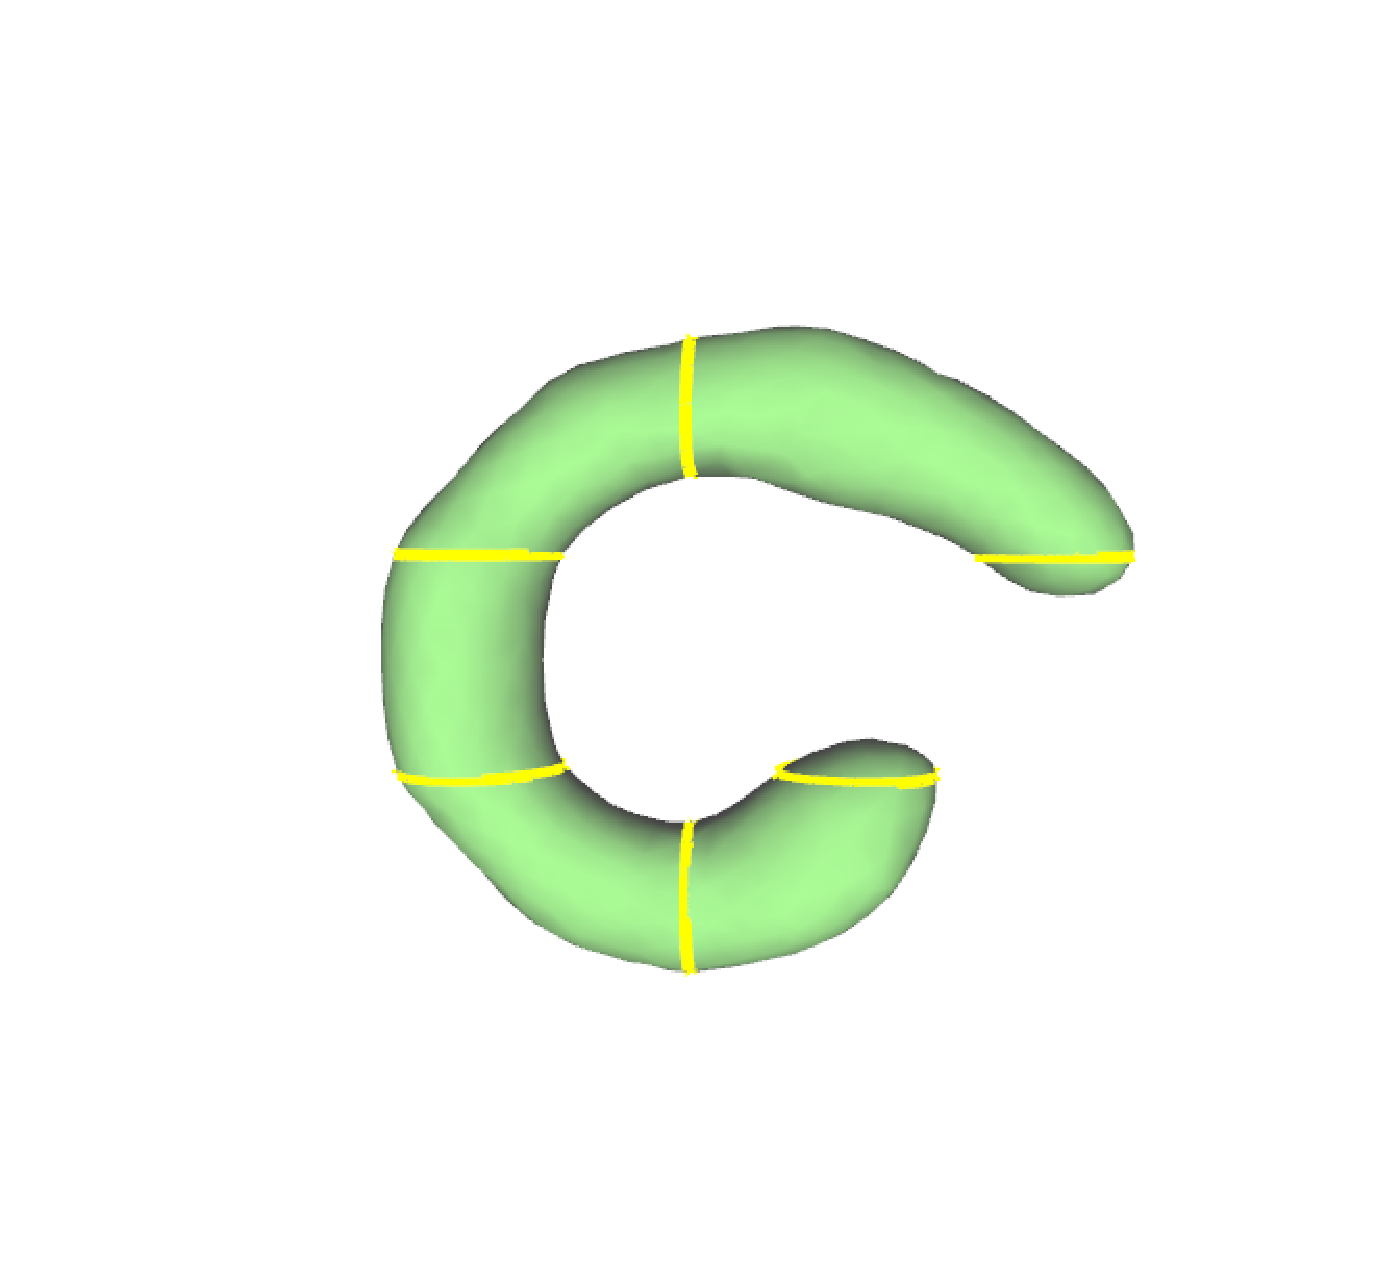
\includegraphics[scale=0.18]{figs/f3.surf-cshape-8.eps}
    \end{minipage}}
  \caption{An example of surface reconstruction from non-intersected cross sections in the \textit{body} zones. (a) The input cross sections; (b) Partition result. The red planes are the bounding planes of each zone and the numbers represent the indices of the zones; (c)-(d) Cylinders generated from the two cross sections in Zone 1; (e) The union of cylinders in Zone 1; (f) The unions of cylinders in all zones; (g) The initial reconstruction result obtained by stitching surfaces in all zones; (h)-(i) The results after 2 and 5 iterations of refinement and
  smoothing. (j) The final reconstruction result after 10 iterations of refinement and smoothing.}
  \label{fig:cshape} %% label for entire figure
\end{figure*}

%no intersection case
For a cross section $cs_p$ on face $f_{ij}$ which does  not
intersect with other cross sections in zone $zn_i$, we need to build
a cylinder $cl_p$ taking the 2D region enclosed by $cs_p$ as the
bottom $cl_p^b$. The initial top $cl_p^t$ of $cl_p$ is obtained by
translating $cl_p^b$ along the direction orthogonal to $f_{ij}$ and
pointing towards the inside of $zn_i$. Suppose the height of the
zone is $h_{zn}$ regarding $f_{ij}$ as the bottom face of the zone
(as we have introduced, each zone is a cuboid), the distance of the
translation $h_p$ (the height of $cl_p$) is then computed as:

\begin{equation}
\label{eq:clheight}
h_p = h_{zn}- \epsilon,
\end{equation}
where $\epsilon$ is a small positive number to make sure that the
center of $cl_p^t$ lie within $zn_i$. In this way, the cylinder
$cl_p$ will be totally contained in the zone $zn_i$ and interpolates
the input cross section $cs_p$. An example of the generation of the
cylinders in this case can be found in Figure~\ref{fig:cshape}.


\begin{figure*} [htbp]
  \centering
  \subfigure[]{
    \centering
    \label{fig:csinters:a}
    \begin{minipage}[b]{0.22\textwidth}
      \centering
      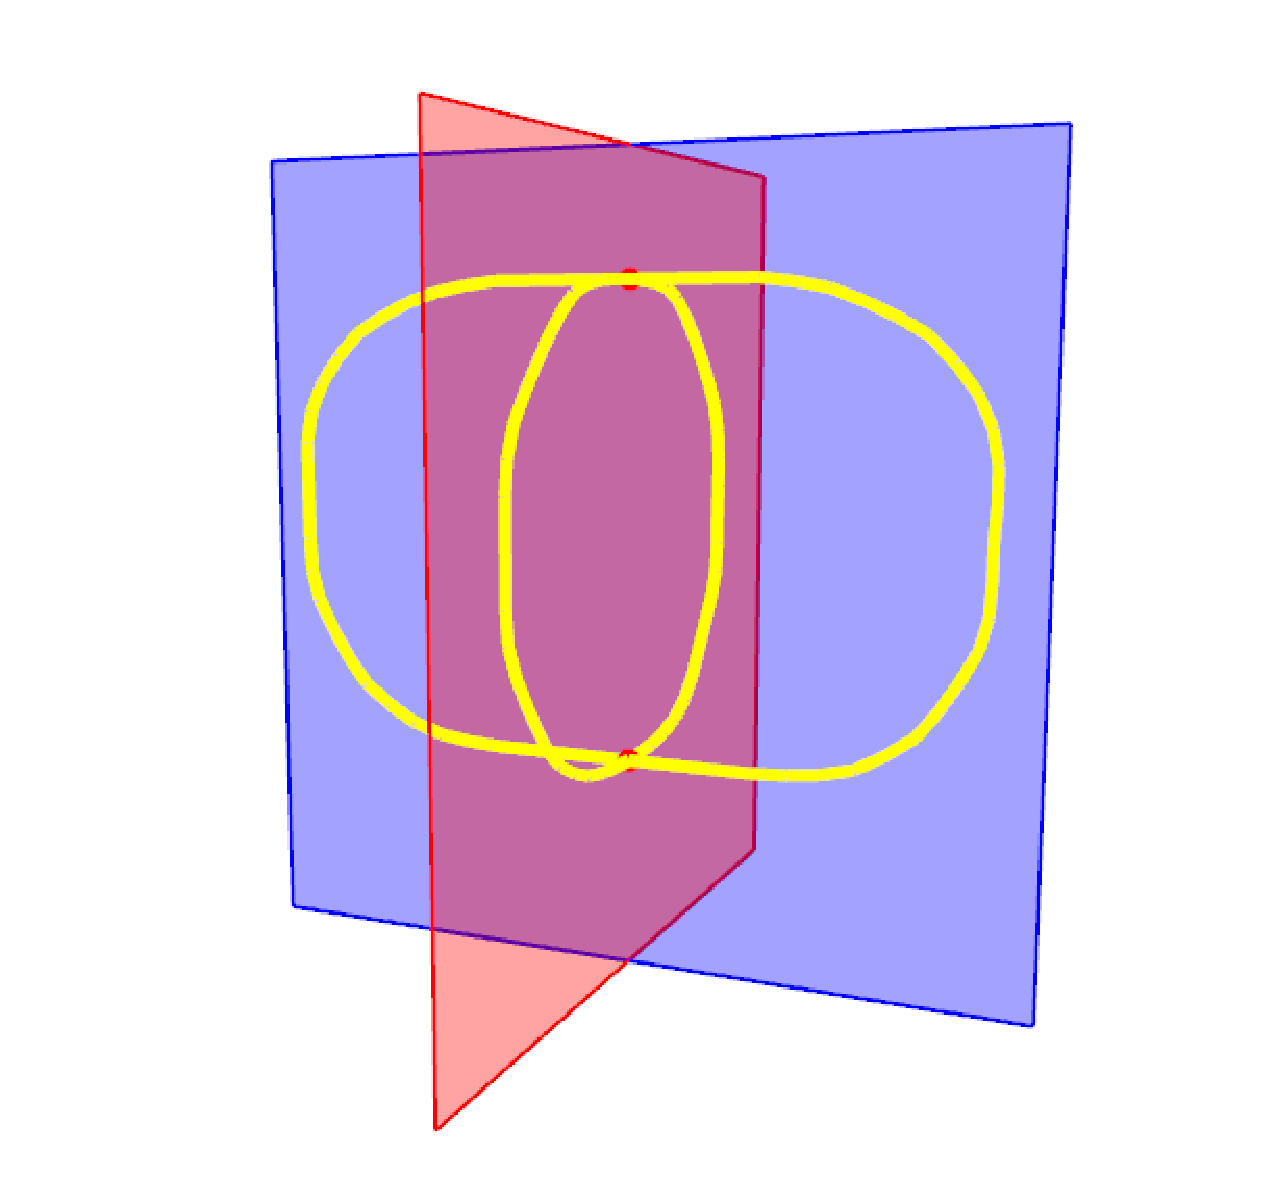
\includegraphics[scale=0.15]{figs/f3.surf-csinters-2.eps}
    \end{minipage}}
  \subfigure[]{
    \centering
    \label{fig:csinters:b}
    \begin{minipage}[b]{0.22\textwidth}
      \centering
      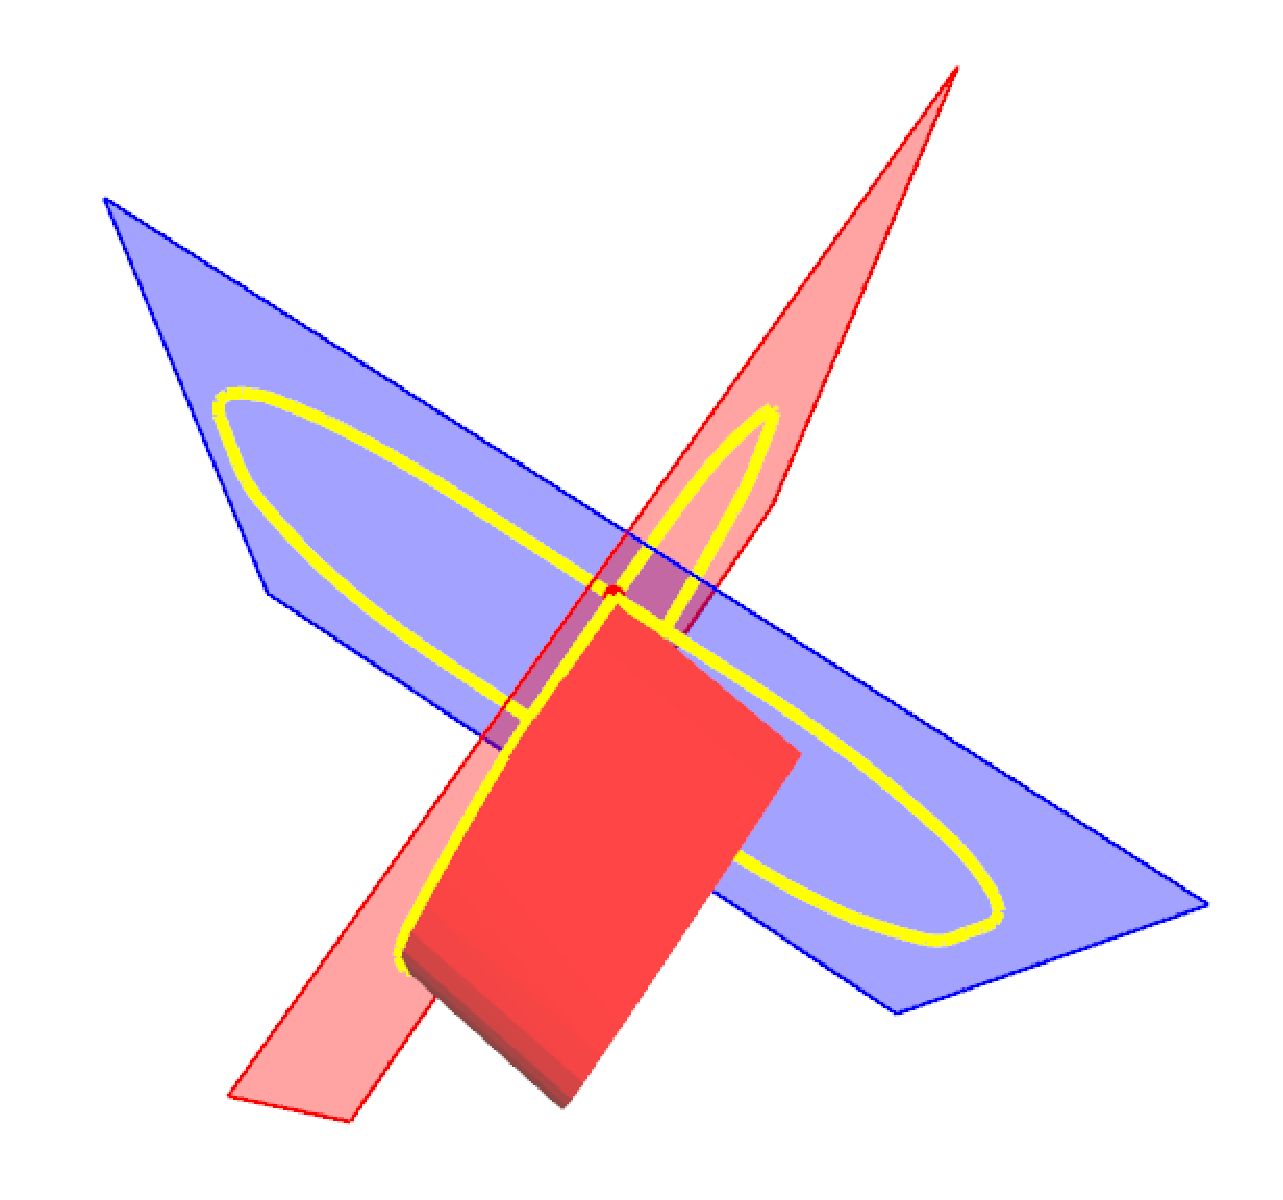
\includegraphics[scale=0.15]{figs/f3.surf-csinters-3.eps}
    \end{minipage}}
  \subfigure[]{
    \label{fig:csinters:c}
    \begin{minipage}[b]{0.22\textwidth}
      \centering
      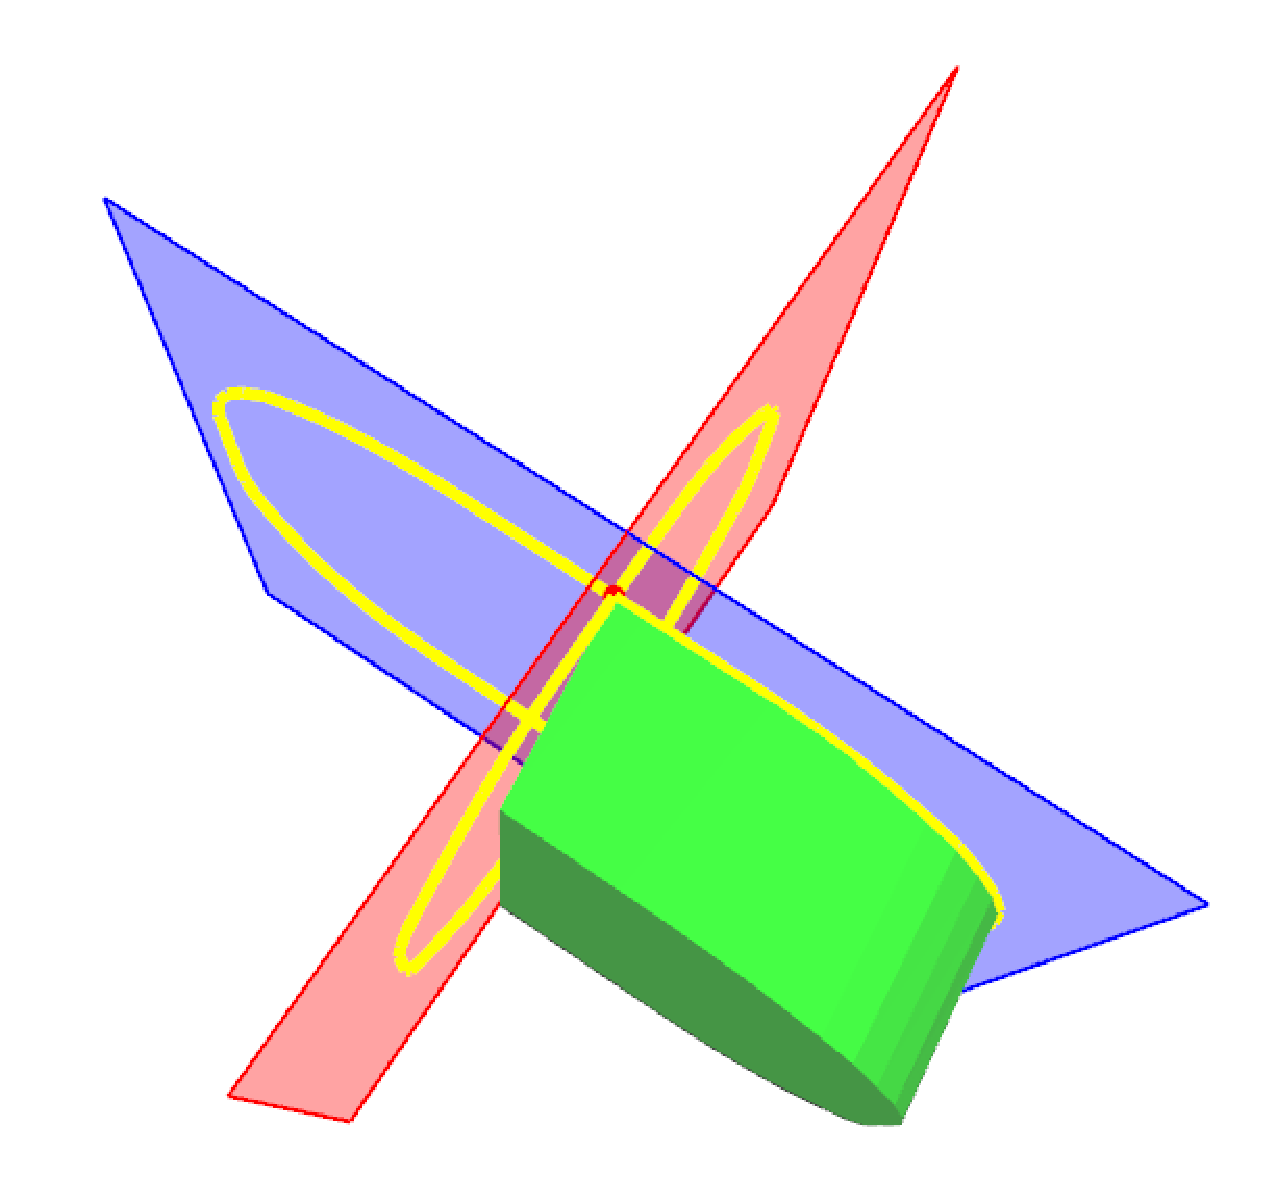
\includegraphics[scale=0.15]{figs/f3.surf-csinters-4.eps}
    \end{minipage}}
  \subfigure[]{
    \label{fig:csinters:d}
    \begin{minipage}[b]{0.22\textwidth}
      \centering
      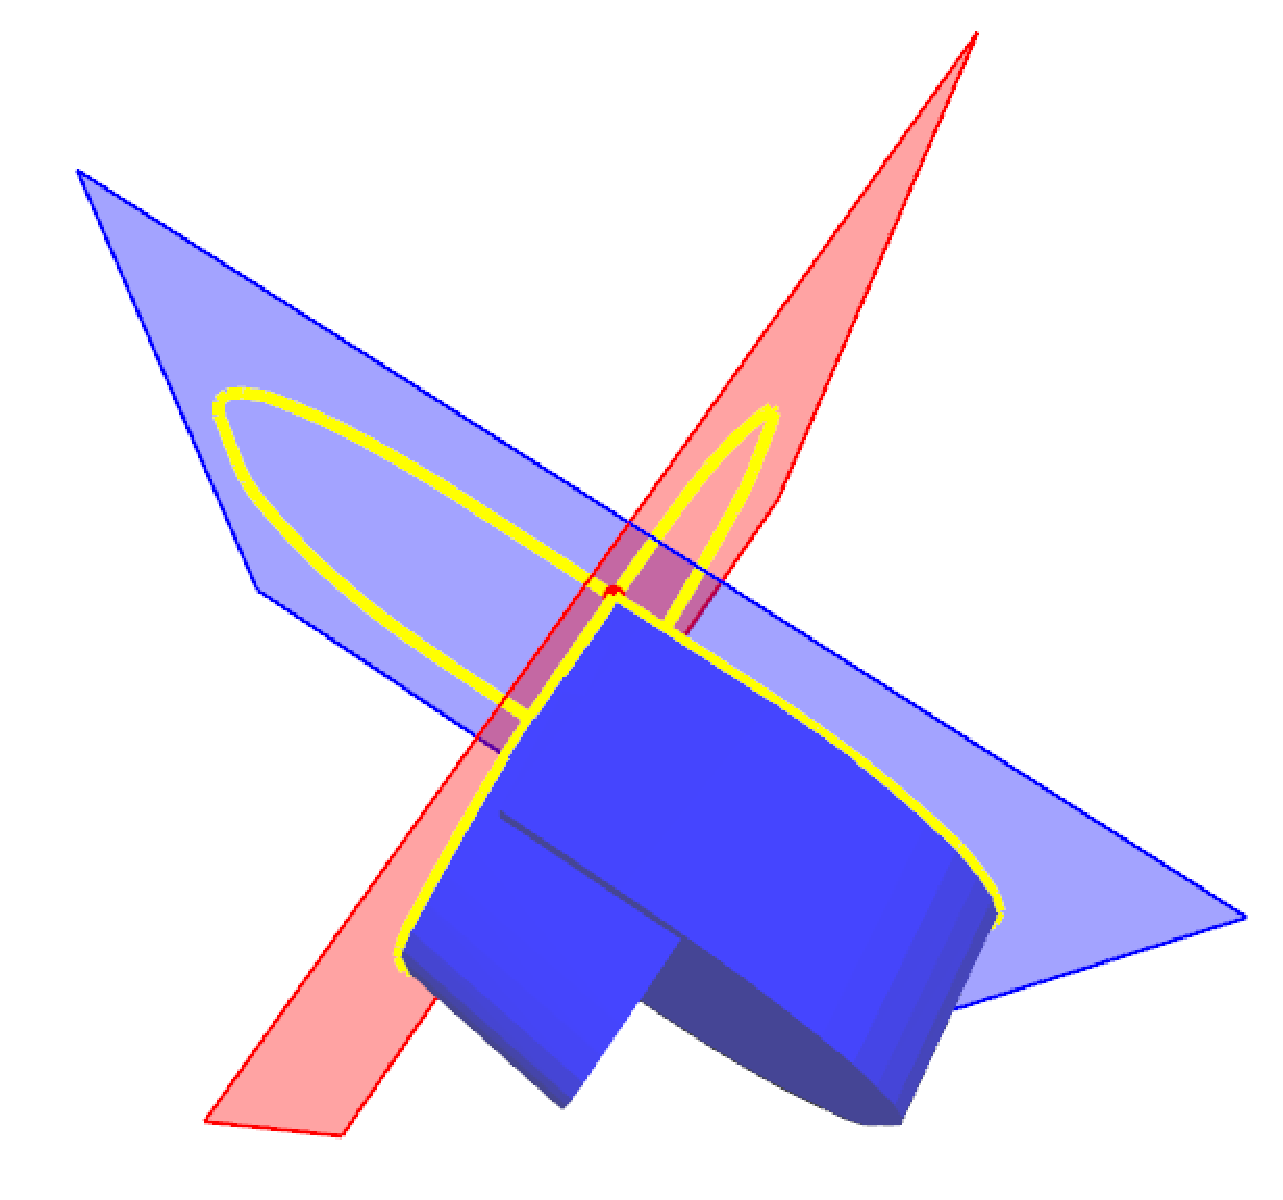
\includegraphics[scale=0.15]{figs/f3.surf-csinters-5.eps}
    \end{minipage}}
  \subfigure[]{
    \label{fig:csinters:e}
    \begin{minipage}[b]{0.22\textwidth}
      \centering
      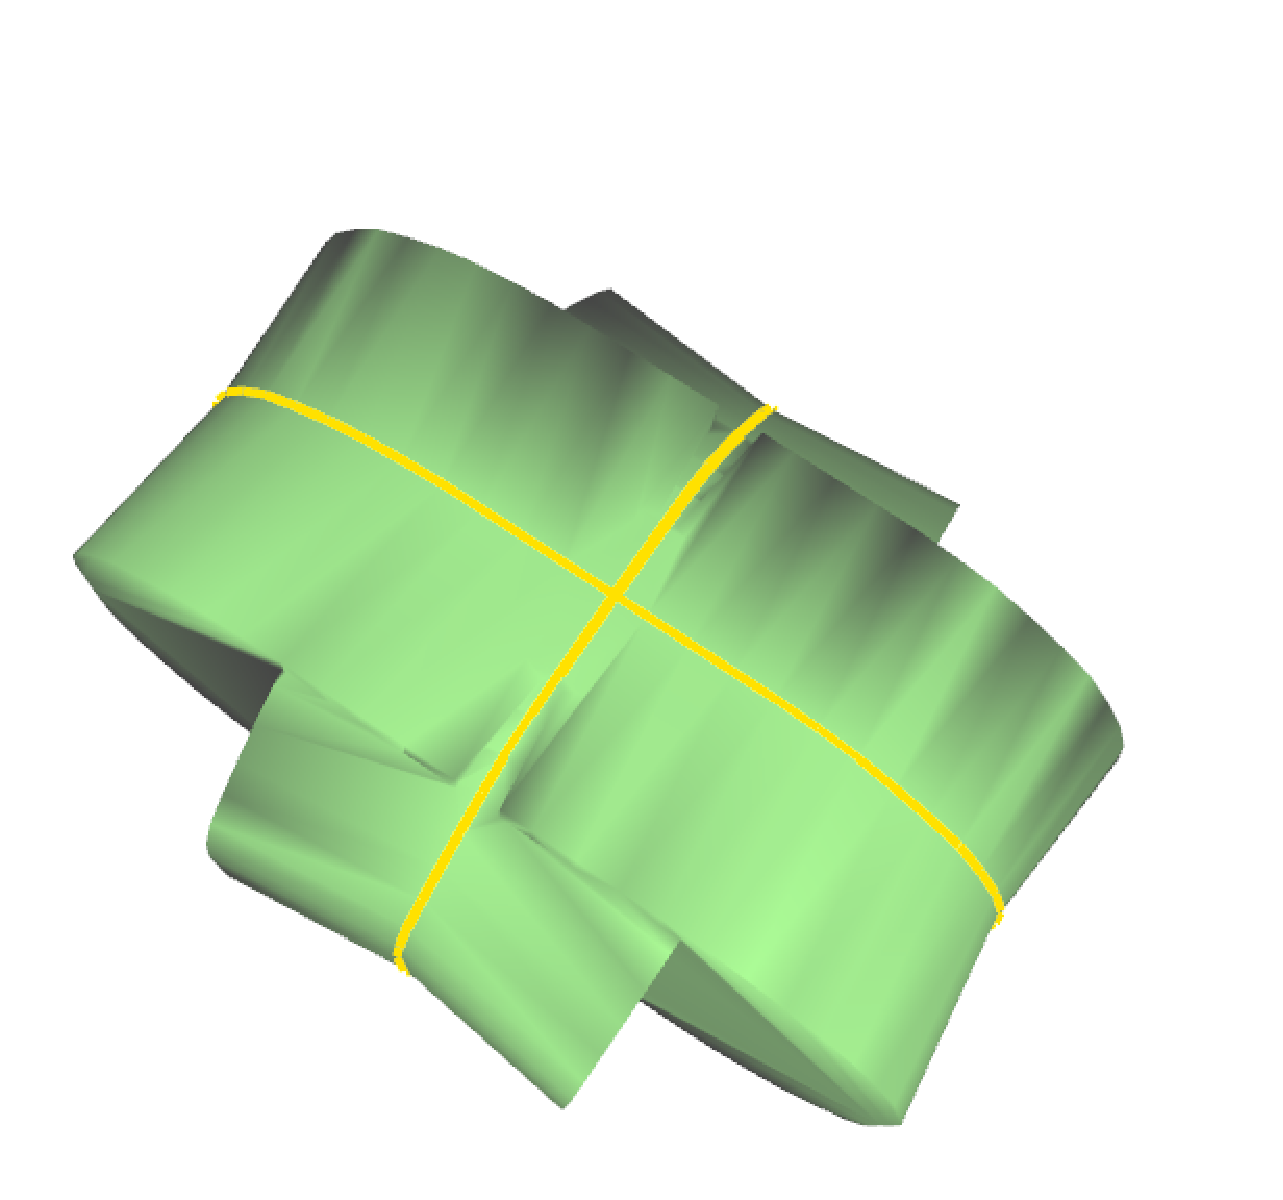
\includegraphics[scale=0.15]{figs/f3.surf-csinters-6.eps}
    \end{minipage}}
  \subfigure[]{
    \label{fig:csinters:f}
    \begin{minipage}[b]{0.44\textwidth}
      \centering
      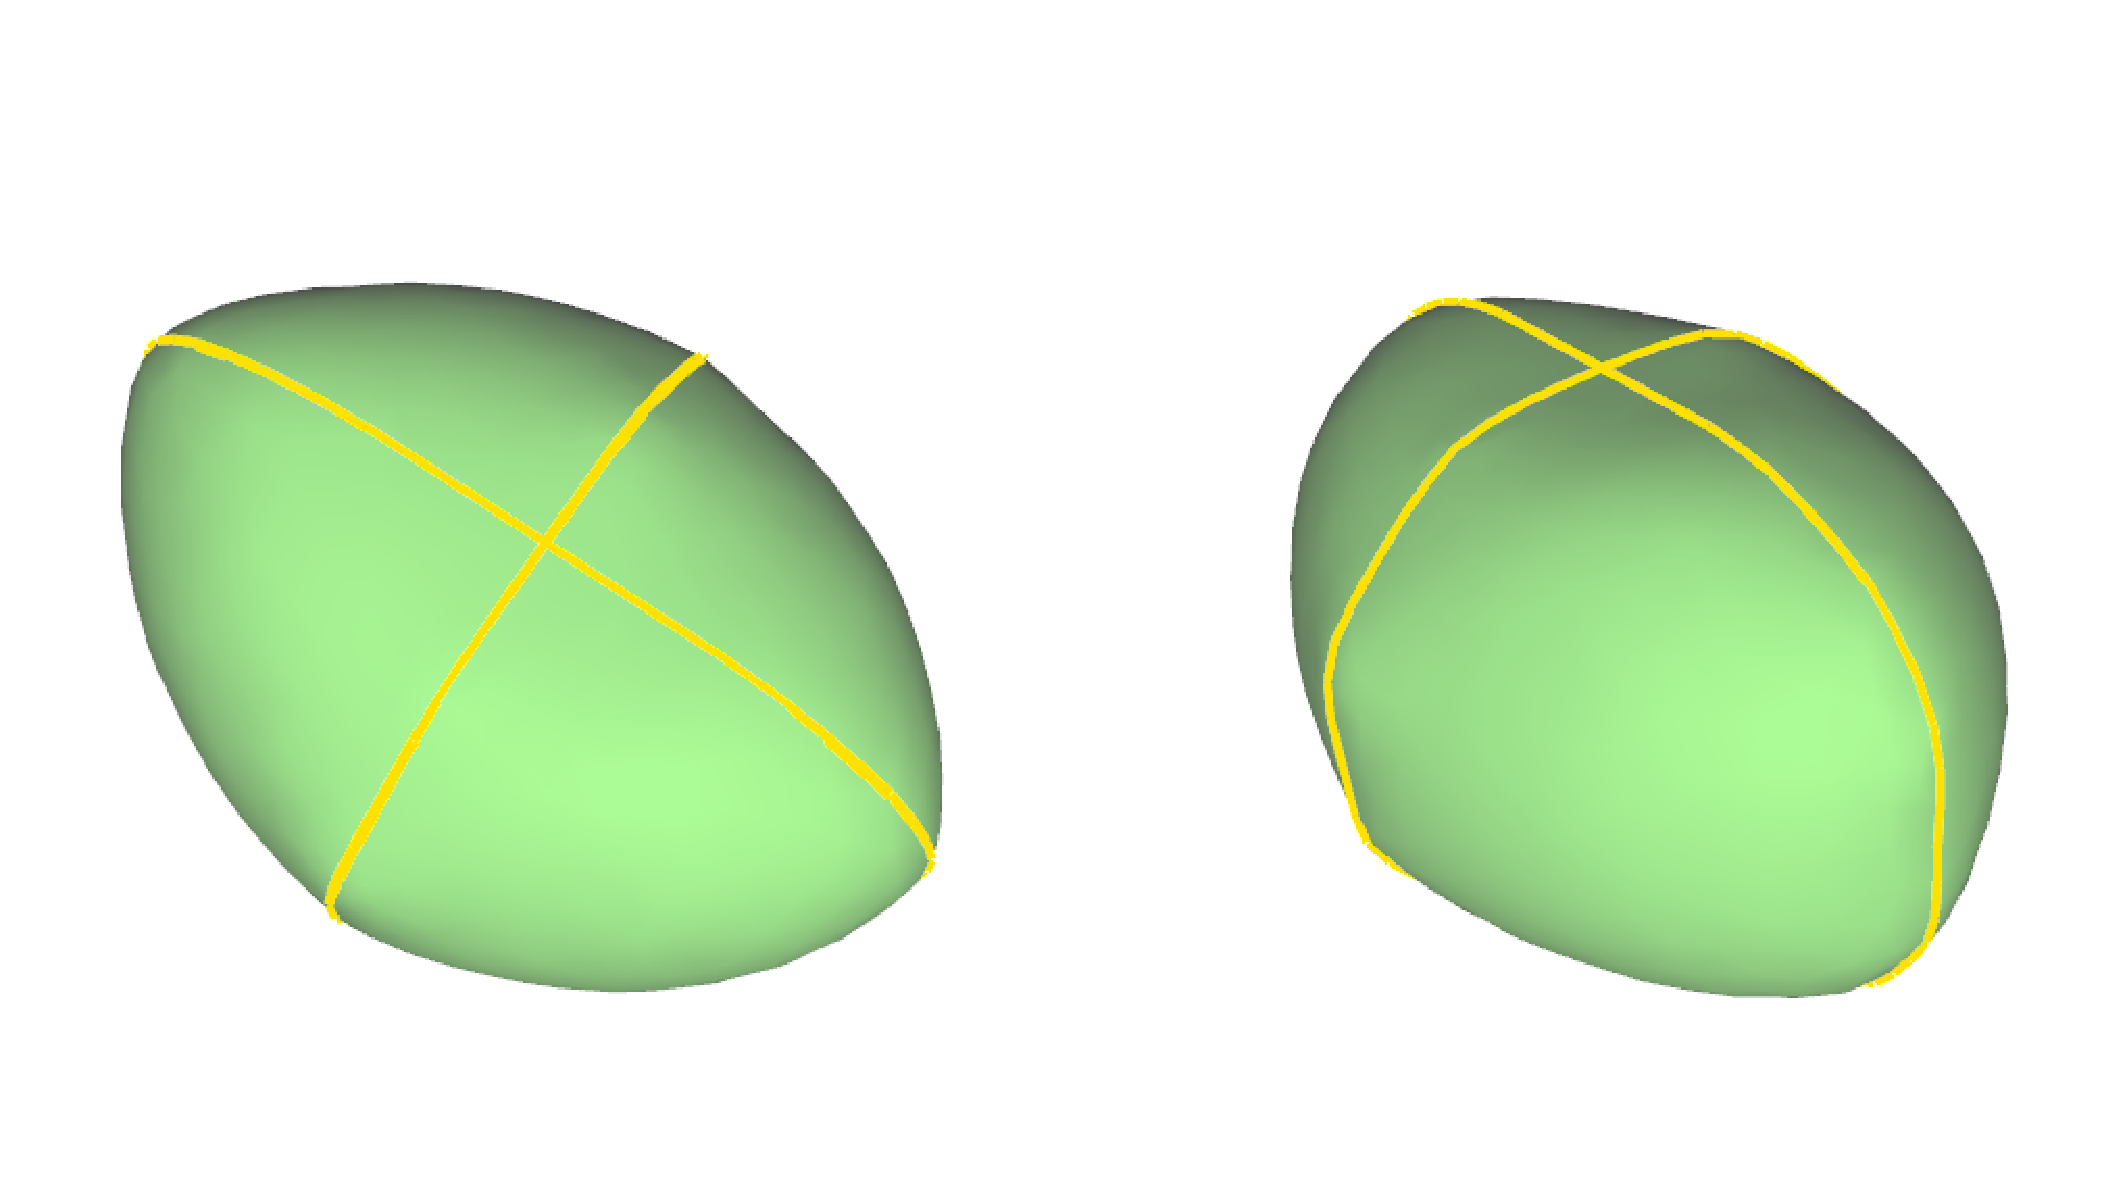
\includegraphics[scale=0.15]{figs/f3.surf-csinters-7.eps}
    \end{minipage}}
  \caption{An example of surface reconstruction from intersected cross sections in the \textit{body} zones. (a) The input cross sections; (b)-(c) Cylinders are generated from the two cross sections and perturbed; (d) The union of cylinders in the zone; (e) The initial reconstruction result; (f) The final reconstruction result after refinement and smoothing.}
  \label{fig:csinters} %% label for entire figure
\end{figure*}

%intersected case, need pertubation
When a cross section $cs_p$ on face $f_{ij}$  intersects with
another cross section $cs_q$ on the neighbor face $f_{ik}$ of
$f_{ij}$ in zone $zn_i$ (see Figure~\ref{fig:csinters:a}), computing
the cylinder $cl_p$ in the above method will make one face of $cl_p$
coincide with $f_{ik}$. As a result, the surface of the union of the
cylinders may probably not interpolate $cs_q$ on $f_{ik}$. In that
case, we first generate an initial cylinder $cl_p^{ini}$ from $cs_p$
in the above method. Then we perturb $cl_p^{ini}$ a little bit, by
translating a subset of points of $cl_p^t$ which lie on the neighbor
face $f_{ik}$ towards the center point of $cl_p^t$ a small distance,
such that there will not be any face of the result cylinder
$cl_p^{ptb}$ coincide with $f_{ik}$, and interpolation of the final
surface on $cs_q$ can thus be achieved. An illustration of this perturbation
process can be found in Figure~\ref{fig:csintersPerturb}. Strictly speaking,
$cl_p^{ptb}$ will not be a cylinder anymore, since the shapes of its
bottom and top are not the same after the perturbation. However,
this will not affect the union calculation which takes general
polyhedrons as input. Similarly, the cylinder $cl_q^{ptb}$ can be
generated from $cs_q$. The result surface after the union
calculation will lie in $zn_i$ and interpolate the input cross
sections (see Figure~\ref{fig:csinters:d}). This perturbation method
also works for the generation of a cylinder from a cross section
which intersects with other cross sections on multiple neighbor
faces.

%%%%%%%%%%%%%%%%%%%%%%%%%%%%%%%%%%%%%%%%%%%%%%%%%%%%%%%%%%%%%%%%%%
%%%%%%%%%added in thesis only
\begin{figure} [htbp]
  \centering
  \subfigure[]{
    \centering
    \label{fig:csintersPerturb:a} %% label for first subfigure
    \begin{minipage}[b]{0.3\textwidth}%\textwidth   %\linewidth
      \centering
      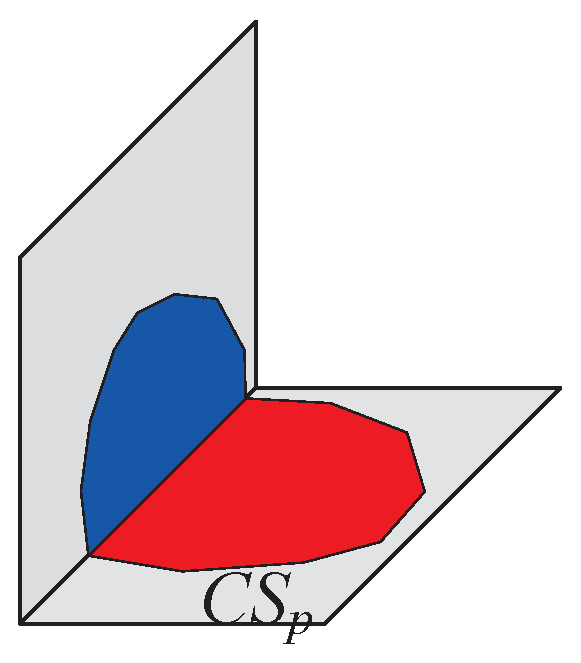
\includegraphics[scale=0.33]{figs/f4.illu-non-intsct-per1.eps}%0.25
    \end{minipage}}
  \subfigure[]{
    \centering
    \label{fig:csintersPerturb:b}
    \begin{minipage}[b]{0.3\textwidth}
      \centering
      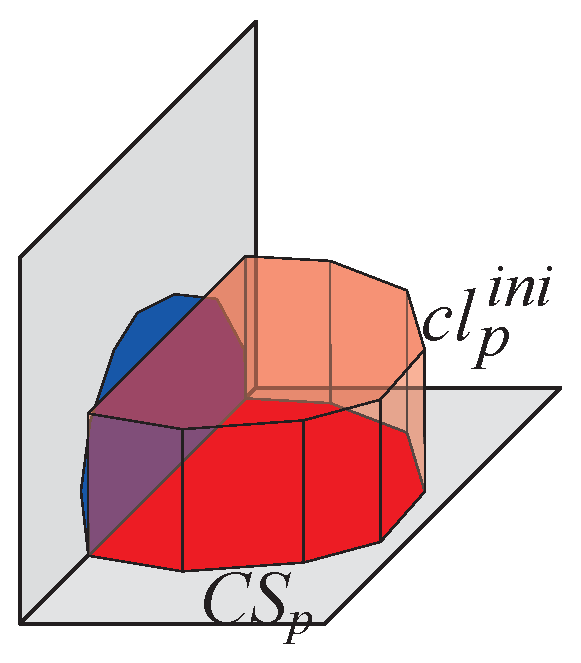
\includegraphics[scale=0.33]{figs/f4.illu-non-intsct-per2.eps}
    \end{minipage}}
  \subfigure[]{
    \label{fig:csintersPerturb:c}
    \begin{minipage}[b]{0.3\textwidth}
      \centering
      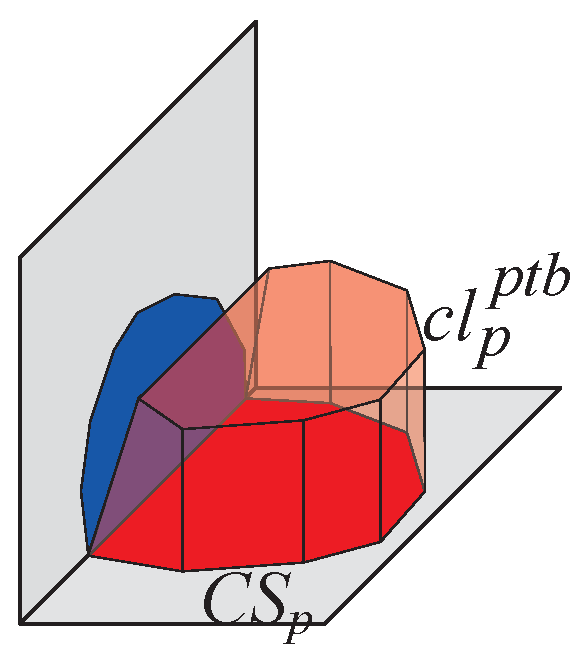
\includegraphics[scale=0.33]{figs/f4.illu-non-intsct-per3.eps}
    \end{minipage}}
  \caption{Illustration of constructing a cylinder for intersected cross sections
  in a \textit{body} zone.
  (a) Input cross sections;
  (b) Generate initial cylinder $cl_p^{ini}$ from one cross section $cs_p$. It can be 
  seen that the other cross section is covered by $cl_p^{ini}$;
  (c) Perturb the top of $cl_p^{ini}$ a little bit, such that the result cylinder
  $cl_p^{ptb}$ will lie within the zone and interpolate $cs_p$.}
  \label{fig:csintersPerturb}
\end{figure}
%%%%%%%%%added in thesis only
%%%%%%%%%%%%%%%%%%%%%%%%%%%%%%%%%%%%%%%%%%%%%%%%%%%%%%%%%%%%%%%%%%


\section{Sub-surface reconstruction for an \textit{end} zone}
\label{ch4:sec:algo:end}

%drawback of existing methods
Similar to the method in~\cite{LBDLJ08}, we use  the classical
partition method in Computational Geometry to divide the whole space
into zones and build sub-surfaces within each zone. However, this
strategy may cause the reconstructed model to have some isolated
components, because some faces which do not have cross sections on
will still take effect on forming the \textit{end} zones (the blue
faces in Figure~\ref{fig:partition:c}), and the cylinders generated
in these zones cannot connect to any other surface components except
those generated in the other incident zones of the faces containing
the cross sections. As a result, these cylinders may probably become
isolated surface components and the whole surface will thus be
composed of multiple components(see the 2D example in
Figure~\ref{fig:workflow2dortho:d} and 3D example in
Figures~\ref{fig:partition:f}).

In progressive modeling, when the user  gradually adds new sketches
that are closely related to the existing shape, the algorithm is
desired to produce a model with only one component. This is a
reasonable criterion that agrees with user's expectation. Therefore,
we adopt a strategy to extend the cylinders built in the
\textit{end} zones to other non-end zones (the \textit{body} and
\textit{empty} zones), to minimize their possibility of becoming
isolated surface components.

%detailed method
Specifically, for each cross  section $cs_p$ on face $f_{ij}$ in an
\textit{end} zone $zn_i$, we first build a cylinder $cl_p$ from
$cs_p$ using the same method as generating a cylinder from a
non-intersected cross section in a \textit{body} zone. Then we check
if the face $f_{ik}$ opposite to $f_{ij}$ in $zn_i$ belongs to the
bounding box or not. If yes, then the extension will be considered
as impossible and $cl_p$ will be treated as the surface component
generated from $cs_p$ in $zn_i$.

If $f_{ik}$ does not belong to the bounding box, the extension is
regarded as possible. In that case, $cl_p$ will be stretched into
the neighbor zone $zn_k$ of $zn_i$ that $f_{ik}$ incident to, along
the direction orthogonal to $f_{ij}$. The height of the $cl_p$ will
then taken as that of the zone $zn_i$ (regarding $f_{ij}$ as the
bottom), plus the computed height in zone $zn_k$ using
Eq.~\ref{eq:clheight} (regarding $f_{ik}$ as the bottom). If the
zone $zn_k$ is a body zone, or the face opposite to $f_{ik}$ in
$zn_k$ belongs to the bounding box, this extension process will
terminate and the extended $cl_p$ will be regarded as the surface
components generated from $cs_p$; Otherwise, $cl_p$ will be further
extended in the same way until these requirements are satisfied.

\begin{figure*} [htbp]
  \centering
  \subfigure[]{
    \centering
    \label{fig:partition:a} %% label for first subfigure
    \begin{minipage}[b]{0.3\textwidth}
      \centering
      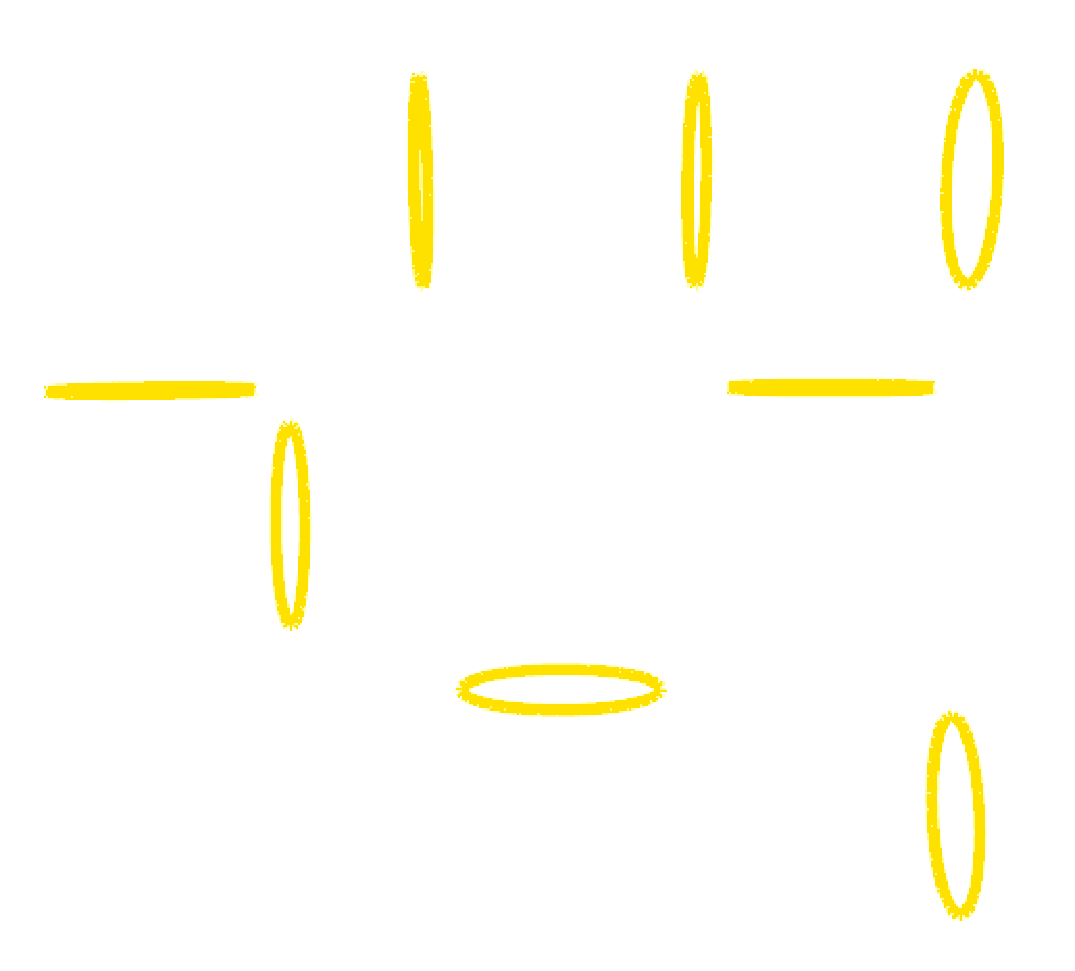
\includegraphics[scale=0.14]{figs/f3.surf-end-1.eps}%0.12
    \end{minipage}}
  \subfigure[]{
    \centering
    \label{fig:partition:b}
    \begin{minipage}[b]{0.3\textwidth}
      \centering
      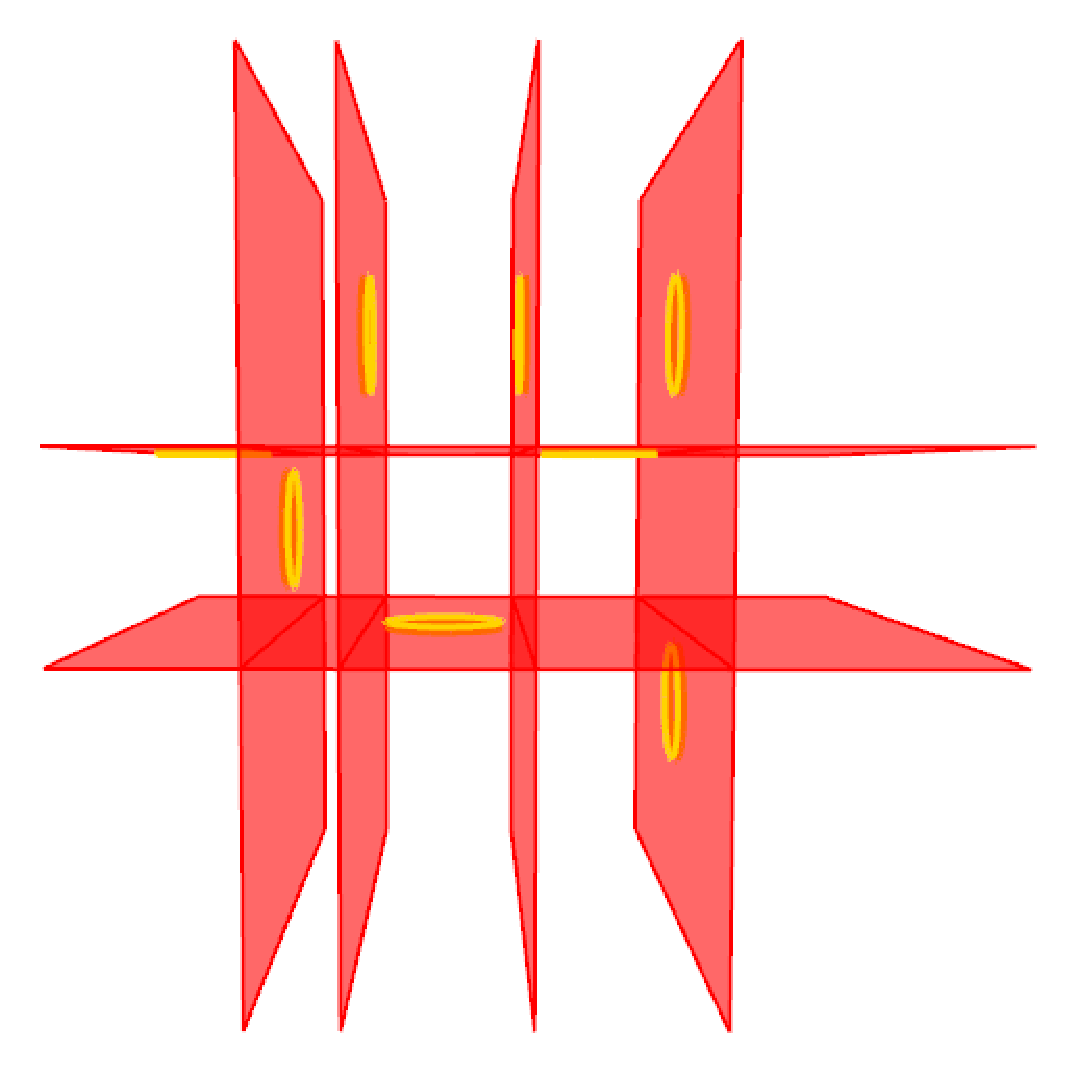
\includegraphics[scale=0.16]{figs/f3.surf-end-2.eps}%0.14
    \end{minipage}}
  \subfigure[]{
    \centering
    \label{fig:partition:c}
    \begin{minipage}[b]{0.3\textwidth}
      \centering
      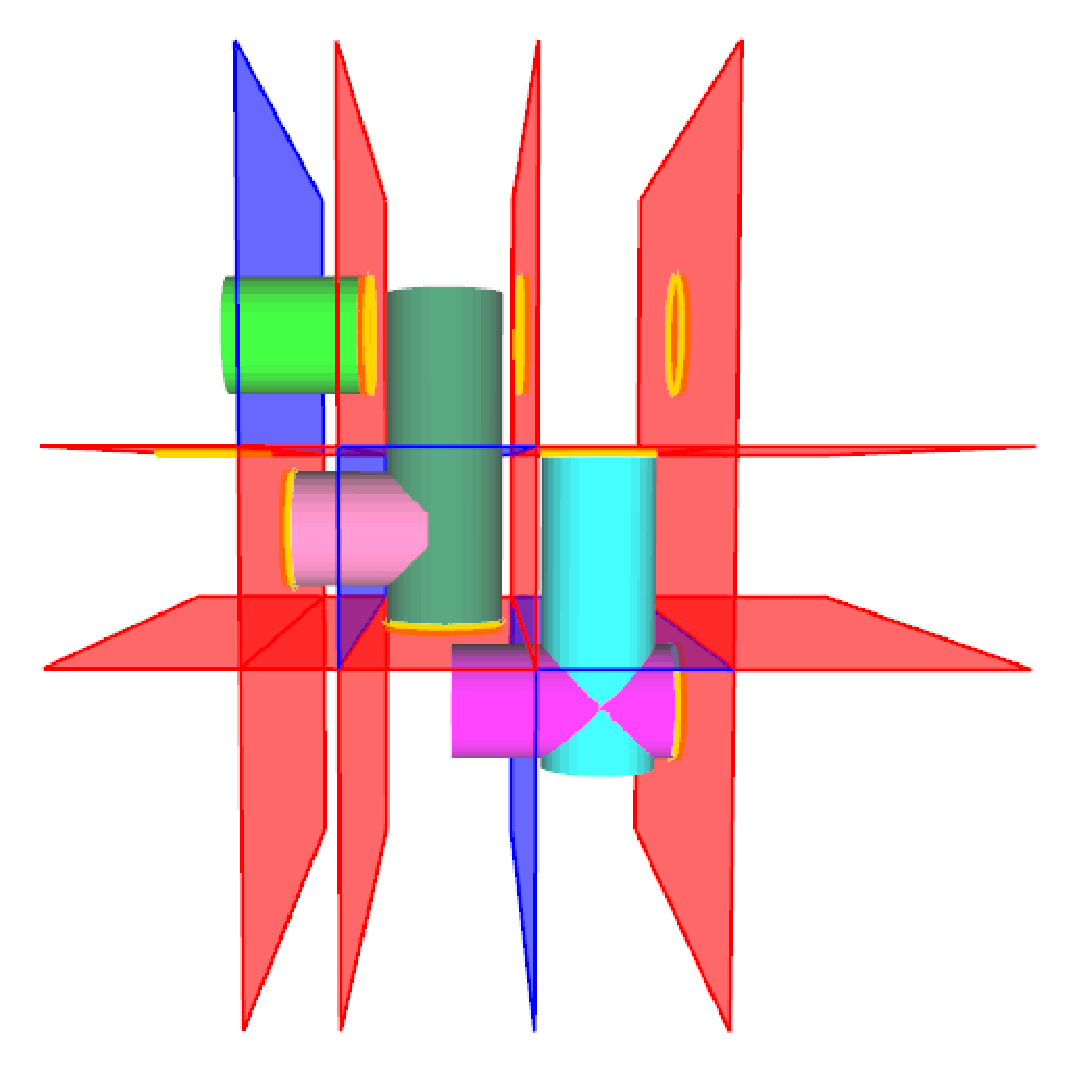
\includegraphics[scale=0.16]{figs/f3.surf-end-3.eps}%0.14
    \end{minipage}}
  \subfigure[]{
    \centering
    \label{fig:partition:d}
    \begin{minipage}[b]{0.3\textwidth}
      \centering
      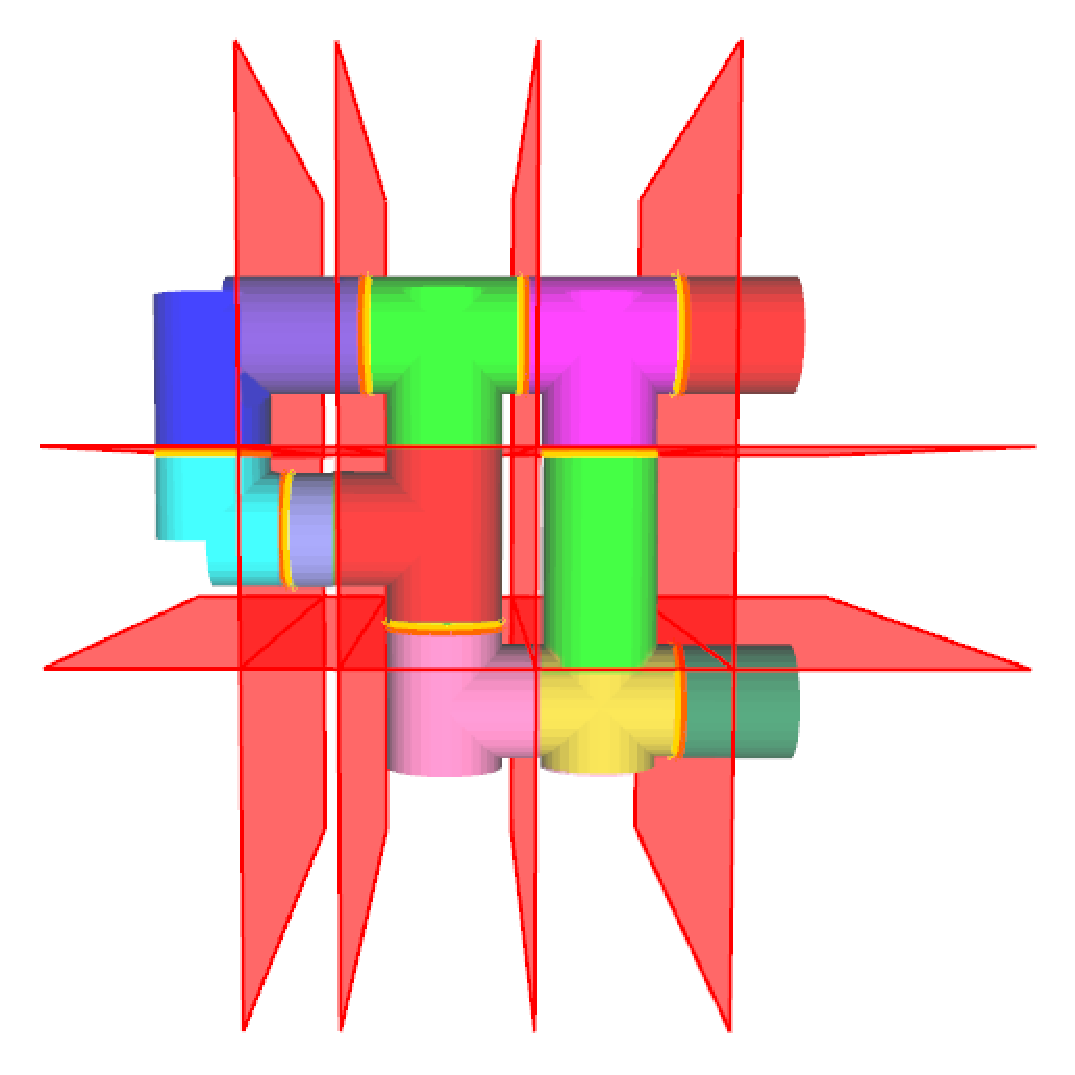
\includegraphics[scale=0.16]{figs/f3.surf-end-4.eps}%0.14
    \end{minipage}}
  \subfigure[]{
    \centering
    \label{fig:partition:e}
    \begin{minipage}[b]{0.3\textwidth}
      \centering
      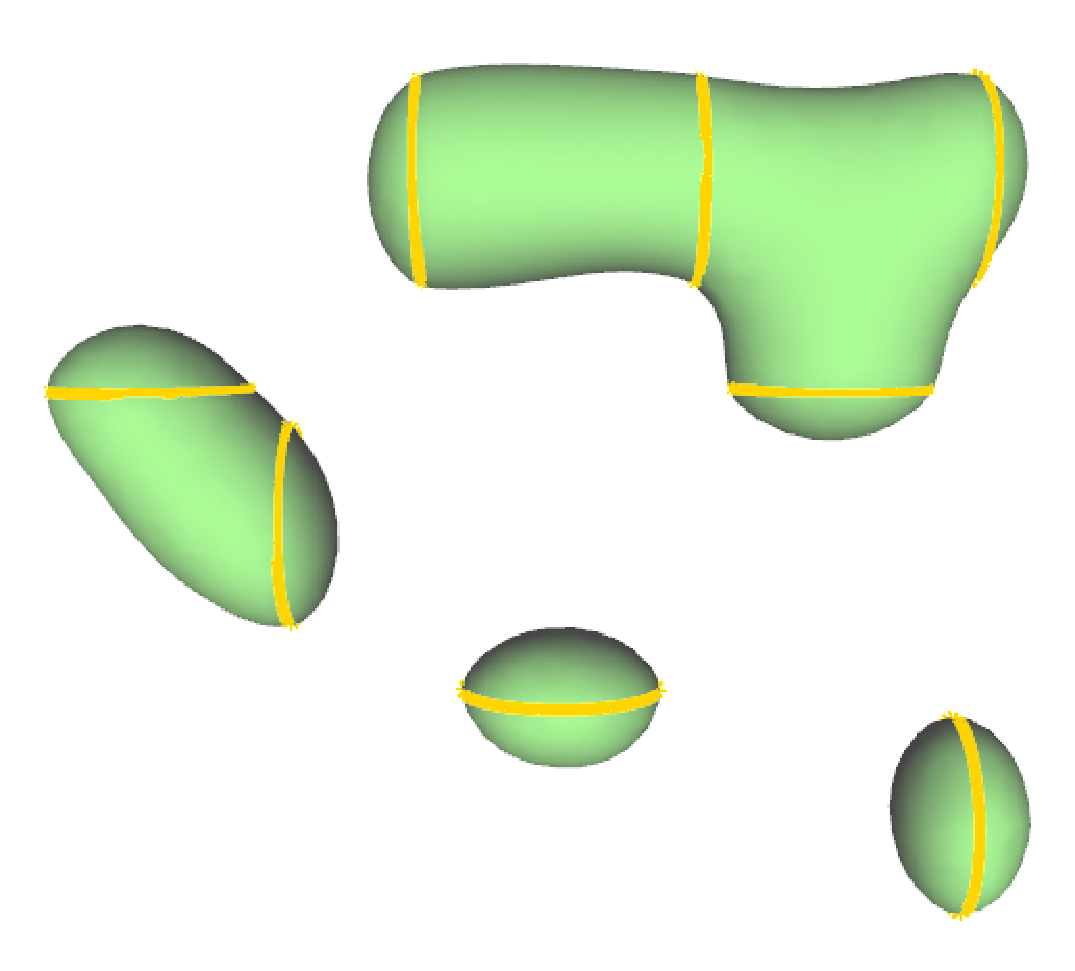
\includegraphics[scale=0.14]{figs/f3.surf-end-5.eps}%0.12
    \end{minipage}}
  \subfigure[]{
    \centering
    \label{fig:partition:f}
    \begin{minipage}[b]{0.3\textwidth}
      \centering
      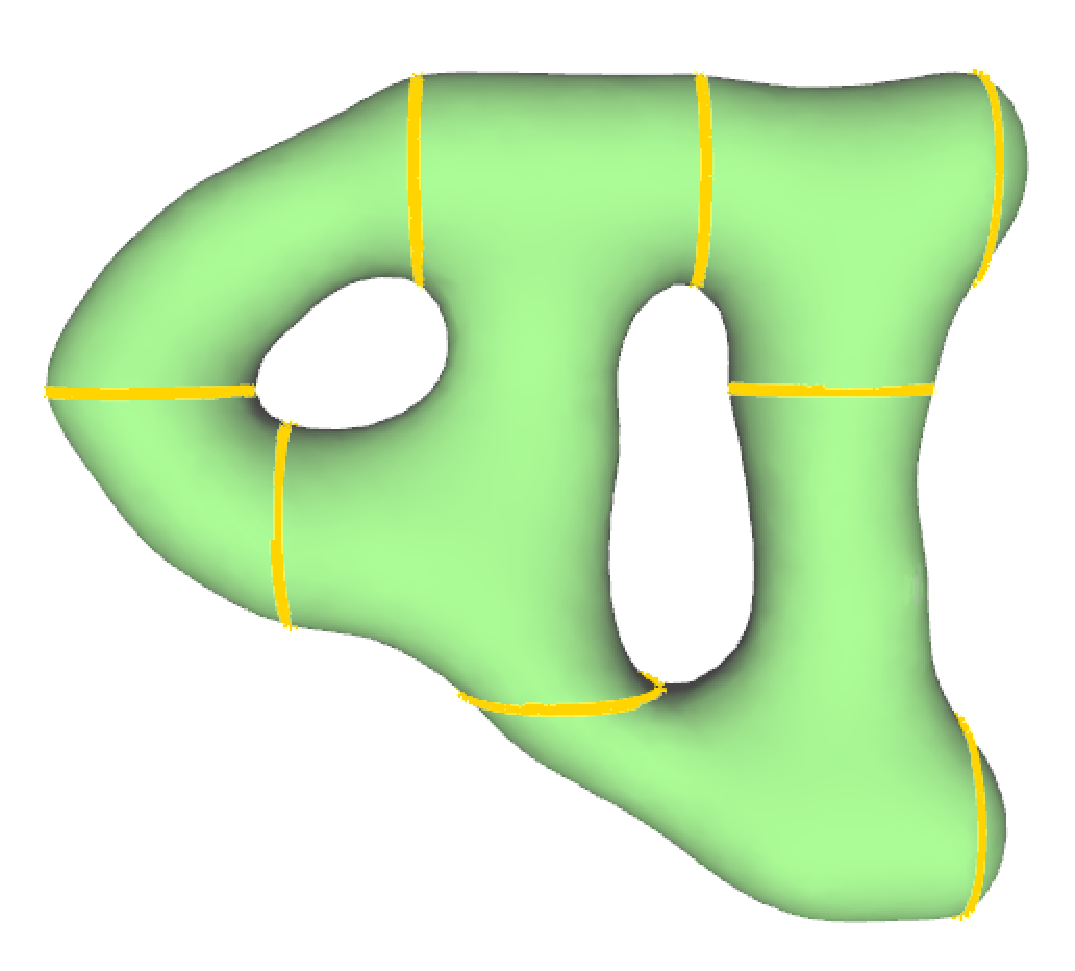
\includegraphics[scale=0.14]{figs/f3.surf-end-6.eps}%0.12
    \end{minipage}}
  \caption{An example of surface reconstruction in the \textit{end} and \textit{body} zones. (a) Input cross sections; (b) The partition result; (c) The extended cylinders for the \textit{end} zones.  The blue faces are those which may cause isolated surface components; (d) The unions of cylinders in all zones; (e) Final surface reconstruction result in our approach; (f) Reconstruction result using the algorithm in~\cite{LBDLJ08}.}
  \label{fig:partition} %% label for entire figure
\end{figure*}

As shown in Figure~\ref{fig:partition}, by extending the cylinders
built in the \textit{end} zones to make them intersect with other
cylinders, isolated surface components can be connected to form a
single component. While for the projection-based method
in~\cite{LBDLJ08}, this extension is not easy to implement, and the
result surface will contain multiple isolated components.

%isolated part cannot be totally eliminated
It should be pointed out that this cylinder extension  strategy
cannot guarantee the final surface to always have a single
component. Such cases may happen when cylinders within the same zone
cannot intersect whatever their heights are (such as the two
cylinders in Zone 6 in Figure~\ref{fig:cshape:f}). Although this
problem can be fixed by changing the shape of the cylinders to force
them connect regardless of the positions of the sketched cross
sections, we do not launch such a process since it may produce
irregular and undesired local shapes. Meanwhile, since the user
usually tends to add a new sketch that is closely related to the
current shape, if an isolated part is to be generated during the
sketching process, a hint will be given to the user to indicate that
possibility caused by the newly added sketch.


\section{Global surface reconstruction} \label{ch4:sec:algo:global}

%After all the cylinders in each zone are built, we use the algorithm
%proposed in~\cite{LTH86} to compute the union of them. The algorithm
%computes the unions of the input polyhedrons by getting those of the
%faces and glue them together, and it is robust and quick enough for
%our application since the shape of the polyhedrons are regular. The
%global surface of the initial mesh $M_{init}$ can then be calculated
%as:

%%%%%%%%%%%%%%%%%%%%%%%%%%%%%%%%%%%%%%%%%%%%%%%%%%%%%%%%%%%%%%%%%%
%%%%%%%%%added in thesis only
After all the cylinders in each zone are built, we use the
CarveCSG library~\cite{CarveCSG} which implements the algorithm proposed
in~\cite{LTH86} to compute the union of these polyhedrons one by one.

Given two polyhedrons $P_a$ and $P_b$, each triangle $Tr^a_i$ on $P_a$ will be
visited first. If $Tr^a_i$ intersects with a triangle $Tr^b_j$ on $P_b$, then
both $Tr^a_i$ and $Tr^b_j$ will be bisected by the plane of each other's.
This way, $P_a$ and $P_b$ will become new polyhedrons $P^\prime_a$ and
$P^\prime_b$ which are composed of bisected triangles. Next, the triangles on
$P^\prime_a$ which are inside the volume of $P^\prime_b$, as well as
those on $P^\prime_b$ inside the volume of $P^\prime_a$ will be removed.
Finally, the left triangles from $P^\prime_a$ and $P^\prime_b$ will
be merged and the union result can be obtained.

This method is robust and quick enough for our application since the shape
of the polyhedrons are regular. The global surface of the initial mesh
$M_{init}$ can then be calculated as:
%%%%%%%%%added in thesis only
%%%%%%%%%%%%%%%%%%%%%%%%%%%%%%%%%%%%%%%%%%%%%%%%%%%%%%%%%%%%%%%%%%


\begin{equation}
\label{eq:surfreconstortho}
    M_{init}=\sum\limits_{i=1}^m {(Cl_{i1} \bigcup Cl_{i2} \bigcup {...} \bigcup Cl_{in})}
\end{equation}
where $Cl_{ij}$ refers to the $j$th cylinder built in  the $i$th
zone, assuming there are totally $m$ zones and $n$ cylinders in each
zone.

\subsection{Mesh improvement}
\label{ch4:sec:algo:global:improve}

Since the shape of the initially reconstructed surface $M_{init}$ is usually unnatural and jaggy, we then improve it through iterative refinement and smoothing.

%%%%%%%%%%%%%%%%%%%%%%%%%%%%%%%%%%%%%%%%%%%%%%%%%%%%%%%%%%%%%%%%%%
%%%%%%%%%modified in the revised thesis
For the mesh refinement, we used the algorithm proposed in~\cite{LP03} to produce a result similar to the Delaunay-like triangulation through iterative triangle splitting and edge swapping.

First, we compute a length attribute $\sigma_i$ for each vertex $v^0_i$ on the input cross sections as the average length of all the edges adjacent to $v^0_i$. Then the attribute for
each neighbor vertex $v^1_i$ which is not on the input cross sections will
be computed as the average of $\sigma_i$ of all $v^0_i$s which are neighbors of $v^1_i$.
The length attributes for all other vertices will be computed ring by ring in
this propagation way.

Then, for each triangle $(v_i, v_j, v_k)$, we compute its centroid $v_c$ and the
length attribute $\sigma_c$ for $v_c$ as
$\sigma_c= (\sigma_i + \sigma_j + \sigma_k)/3$. For any vertex $v_m$ ($m \in \{i,j,k\}$)
of this triangle, if $\alpha ||v_m-v_c||> \sigma_c$ and $\alpha ||v_m-v_c||> \sigma_m$
(we set $\alpha=\sqrt{2}$ as suggested in~\cite{LP03}),
we split the triangle $(v_i, v_j, v_k)$ to triangles $(v_i, v_j, v_c)$,
$(v_j, v_k, v_c)$ and $(v_k, v_i, v_c)$, and relax the edges $(v_i, v_j)$, $(v_j, v_k)$
and $(v_k, v_i)$.

Here relaxing an edge $(v_i, v_j)$ means for the two triangles $(v_i, v_j, v_k)$ and
$(v_i, v_j, v_n)$ adjacent to $(v_i, v_j)$, we check if $v_k$ and $v_n$ lie inside
the circumcircles of triangles $(v_i, v_j, v_n)$ and $(v_i, v_j, v_k)$ respectively.
If yes, we implement the edge swapping to let the two triangles become
$(v_i, v_k, v_n)$ and $(v_j, v_k, v_n)$. To ensure the interpolation on the input curves,
the edge swapping is restricted to the edges which do not belong to the input cross sections.

If there are new triangles created in the triangle splitting step, we relax all the edges
on the mesh surface and repeat the splitting step; otherwise, the refinement process is complete.


For the mesh smoothing, we adopted the algorithm in~\cite{YB02} to produce meshes
with smooth shapes. The position $p_i$ of each vertex $v_i$ is updated to $p^\prime_i$
through the following equation:

\begin{equation}
\label{eq:surfsmooth}
    p^\prime_i = p_i + \tau_i N_i + \epsilon_i T_i.
\end{equation}
In the above equation, $N_i$ is the unit normal vector at $v_i$. We compute $N_i$
as the normalized weighted sum of the normals of the incident triangles of $v_i$,
with weights equal to the areas of the triangles. We set the factor
$\tau_i = A_i^2/150$ as suggested in~\cite{YB02}, where $A_i$ is the minimum area
among all the incident triangles of $v_i$. To improve the stability of the surface
evolution, we then move the vertex along a tangential vector $T_i$ to make
the triangle sizes as equal as possible. More precisely, we compute it
as $T_i = \delta_i + N_i$, where $\delta_i$ is the vector pointing from $v_i$
to the centroid of all its neighbor vertices. The factor $\epsilon_i$
is set to $0.5$ in Eq.~\ref{eq:surfsmooth}. Similarly, the position update is only
limited to the vertices which do not lie on the input cross sections
to ensure the interpolation.

%The initial surface is evolved by first moving each vertex along its normal direction to minimize the local curvature differences. Then to improve the computational stability, the triangle sizes are made as equal as possible by moving the vertices along the tangential direction. These two movements are implemented iteratively on the vertices that do not lie on the input cross section curves.

%%%%%%%%%modified in the revised thesis
%%%%%%%%%%%%%%%%%%%%%%%%%%%%%%%%%%%%%%%%%%%%%%%%%%%%%%%%%%%%%%%%%%

In our implementation, we alternatively refine and smooth the initial mesh for 10 iterations. The result surface will have satisfactory quality and its interpolation on the input cross sections is maintained. An example of the
refinement and smoothing process can be found in Figure~\ref{fig:cshape}.


%=================section==================
\section{Results and discussions}
\label{ch4:sec:disc}
%==========================================

%advantage of our method
Examples produced by our sketch-based modeling  system using the
CSG-based progressive surface reconstruction algorithm can be found
in Figure~\ref{fig:models:sketch}.

By making use of the cylinders which reflect the shape and
positions of the sketched cross sections in the reconstruction
process, our approach can get rid of the MA plane, whose change is
more complicated during progressive sketching and will lead to
unexpected shape change of the surface parts generated from
unrelated cross sections. As a result, the change of the model shape
will be natural under any sketching orders, which meets
Requirement~\ref{req:1} for our sketching system. An example showing
this advantage of our CSG-based method over the projection-based
method in~\cite{LBDLJ08} can be found in Figure~\ref{fig:csgma}.

%why order insensitive
In the reconstruction process, the extension of the cylinders in
the isolated zones, as well as the union calculation of the
cylinders in all zones are carried out independently. So for a same
set of sketches, the final reconstruction result will be unique and
insensitive to its input orders.

%other advantages of the CSG-based method, local calculation
There are also some other advantages of the  CSG-based method which
have been utilized in our progressive modeling interface. For
example, since the calculations within each zone are independent,
each time the user adds, modifies or deletes a cross section, only
the sub-surfaces in the affected zones need to be recalculated and
updated, while those in other zones can be retained. In this way,
the calculation can be implemented locally and accelerated.

%partial cross section: stroke rules+subzone+previewed shape and computed cross sections
The independence of calculation in each zone also makes it possible
to allow the sketching of only a part of the cross section instead
of a complete one, as long as the stroke rules are satisfied within
the zone. Since the user sketches are more or less arbitrary, we
also perform automatic curve sewing similar to that mentioned in
Section~\ref{ch3:sec:algo:rule} or give user related hints, to make
sure the stroke rules are followed.

%progressive surface reconstrucion: not only in sbim, but also applications input progressively and require real-time reconstruction result, such as ultra-sound...
Although the CSG-based progressive surface reconstruction  algorithm
is designed for the sketching operation in our system, it can also
be used in other applications such as the CT or ultrasound scan, in
which the input cross sections are obtained from gradually scanned
slices. By making use of our algorithm, the reconstructed 3D model
can be built progressively and its shape can be updated in a natural
manner to provide the user desired real-time feedback.
